\chapter{OPTIMIZING THE SENSITIVITY OF THE $H\rightarrow\mu^+\mu^-$ SEARCH} \label{optimize}

This chapter covers the work to optimize the sensitivity of the analysis. The work on the Level-1 Muon Trigger is covered first, and the classification and categorization of events is covered after. The work on the trigger improves the sensitivity by increasing the amount of data available to the $H\rightarrow\mu^+\mu^-$ search, and the classification and categorization of events groups the events to maximize the chance of discovery.  

\section{Improving The Level-1 Muon Trigger}

Saving as much relevant data as possible is important as the chance of discovery improves with a larger dataset. With this in mind, improvements are made to the L1 Muon Trigger to improve its capability to save events with high momentum muons and discard events without them. Towards this end, Boosted Decision Trees (BDTs) are trained to distinguish high momentum muons from low momentum muons. The BDTs are loaded onto Field Programmable Gate Arrays (FPGAs) in the L1 Muon Trigger and run online. The improvements increase the amount of data with high momentum muons available for the $H\rightarrow \mu^+\mu^-$ search. 

The LHC collides bunches of protons every 25 ns at a center of mass energy of 13 TeV. The CMS experiment detects the resulting particles and measures their kinematics using a variety of subdetectors working in concert. With 40 million proton bunch crossings per second amounting to roughly 40 TB of data each second, saving the information from every event is not feasible. As such, the CMS trigger system chooses the interesting events to save to disk, operating in two stages \cite{Khachatryan:2016bia}. The Level-1 (L1) trigger runs in hardware online reducing the throughput of data from 40 MHz to 100 KHz. From there, the High Level Trigger (HLT) operates in software online reducing the rate from 100 KHz to 1 KHz. In the end, about 1 GB/s is saved to disk.

With 40 MHz of input, the L1 Trigger has only 4 $\mu$s to decide whether to keep the information for an event. The Endcap Muon Track Finder (EMTF) -- part of the L1 Trigger dedicated to muons -- has only about 500 ns to determine the location, tracks, and momentum of the muons passing through the Cathode Strip Chambers (CSC) and Resistive Plate Chambers (RPC) in the endcaps of CMS \cite{Tapper:1556311}. High momentum muons are an important object for many physics analyses at CMS and the most important object for $H\rightarrow\mu^+\mu^-$. As such, an accurate momentum assignment distinguishing low momentum muons (background) from high momentum muons (signal) is key to the L1 Trigger. In order to meet the timing requirements, the EMTF's logic is implemented in Field Programmable Gate Arrays (FPGAs), a type of reprogrammable hardware that allows vast parallelization and speeds much greater than even the best CPUs.

To improve the transverse momentum ($p_t$) assignment for muons in the endcaps at Level-1, the EMTF team trained Boosted Decision Trees (BDTs) offline using TMVA \cite{Hocker:2007ht}, and stored the prediction scheme into a 1.2 GB Look-Up Table (LUT). The FPGAs then use the LUT online to assign the $p_t$ in a single operation. Using the LUT to turn the BDT $p_t$ assignment into a simple look-up enables the EMTF to utilize the power of a robust machine learning algorithm for its momentum predictions while still operating at the required time scale. Putting a parallelized version of the BDTs directly into the FPGAs, while hypothetically possible, would require more than the available number of logic gates. Such an implementation would still be slower than the LUT method, and changing the $p_t$ assignment would require reprogramming the FPGA logic each time. The LUT method provides a simple way to run any machine learning evaluation at high speed by turning the evaluation into a single operation.

\subsection{Metrics Of Success}

Two metrics are used to measure the success of the EMTF: the rate and the efficiency. The rate at X GeV is defined as the number of muons with a predicted $p_t$ greater than X GeV. In other words, the rate consists of both true and false positives above the $p_t$ threshold. The efficiency at X GeV is defined as the number of muons with both predicted $p_t$ and true $p_t$ greater than X GeV divided by the number of muons with true $p_t$ above X GeV. Put another way, the efficiency measures the percentage of muons with true $p_t$ above X GeV correctly predicted above X GeV. A good trigger will minimize the data saved without losing the interesting high $p_t$ events where unexplored physics lies, i.e. it will minimize rate while maximizing the efficiency.

\subsection{The EMTF Regression Project}

A muon traveling through the endcap detectors has a chance to leave hits in four sequential stations labeled 1, 2, 3, and 4. The specific combination of hits like 1,3,4 is called the mode. Each station records the $\phi$ and $\theta$ location of a hit, among other information. The CSCs have better spatial resolution, so the $\phi$ and $\theta$ information is taken from the CSCs by default, but the RPC measurements for the station are used if the CSCs missed the hit in the same station. The charged muons travel through a magnetic field following curved paths due to the Lorentz force. The force causes the high $p_t$ muons in a magnetic field to bend less and the low $p_t$ muons to bend more. The difference in $\phi$ and $\theta$ between stations i and j, $\Delta\phi_{ij}$ and $\Delta\theta_{ij}$, quantify the curvature of the track. With most of the curvature accounted for by the $\Delta\phi$ variables, the $\Delta\phi$s provide the majority of the $p_t$ discrimination.

A major difficulty in minimizing the rate is the steeply falling $p_t$ distribution. A typical interesting event has $p_t$ greater than 25 GeV, and there are about one thousand 5 GeV muons for every 25 GeV muon. With so many more low $p_t$ events, predicting the low momentum muons poorly will drastically increase the rate. Moreover, in addition to the large number of low $p_t$ muons, there are other noteable difficulties: the muons travel through a non-uniform magnetic field, some scatter between detector stations, and those with high $p_t$ often shower charged particles upon interacting with the detector material. Moreover, low $p_t$ muons may spiral completely before getting to the next station. The scattering, showering, and spiraling add noise to the underlying true behavior, while the number of low $p_t$ muons requires that the regression focus on the low momentum regime to prevent an explosion in the rate.

In order to assign $p_t$ in a robust way and deal with the aforementioned difficulties, a BDT is trained for each possible mode using the discretized values for the features of Table \ref{tab:bits}. The loss function and weights are chosen to focus on the low $p_t$ events and minimize the rate while maintaining acceptable efficiency. Features are chosen for each mode to give the BDT the information needed to predict the $p_t$ while dealing with the non-uniform magnetic field and the problematic scattering and showering effects.

The $\Delta\phi$ variables available for each mode are used as features to determine the curvature and get most of the $p_t$ discrimination. However, the power of these variables depends largely on the track position in $\theta$. The magnetic field varies as a function of $\theta$ affecting the magnitude of the curvature for a given $p_t$, thus correlating $\Delta\phi$, $p_t$, and $\theta$. The link between these three makes $\theta$ the next most important training feature.

Variables modeling the mean and RMS of the available $\Delta\phi$s for the mode are also used as features in order to identify scattering and showering effects. If a muon were to scatter or shower between stations the recorded hit in a station may not be the true hit of the muon. Any $\Delta\phi$ involving this station will be an outlier. To determine the severity of the deviation and the likelihood of scattering/showering, the idea is to identify the outlier station and to compare the mean and RMS $\Delta\phi$ with and without the outlier station. The greater the difference the greater the severity. The nominal mean and RMS $\Delta\phi$ features are calculated using all available $\Delta\phi$s for the mode. The exclusive mean and RMS are calculated using all available $\Delta\phi_{ij}$ for the mode with i or j $\neq$ $S_{out}$, where $S_{out}$ is the outlier station. $S_{out}$ is the excluded station such that leaving it out of the sum minimizes the mean and RMS. The outlier station, $S_{out}$, is also used as a feature. Including the nominal mean and RMS of $\Delta\phi$, the exclusive RMS and mean of $\Delta\phi$, and $S_{out}$ as features helps the BDT differentiate scattering, showering, and normal events.

The features described above are the most important features, but not the whole collection. The front-rear (FR) bit designates whether the muon hit a front or rear CSC chamber in the station, and it is also included. The $\Delta\theta$s provide additional curvature information, and these are included as well. The $B$ feature for each station is included as well, and it flags whether the $\phi$, $\theta$ information for the station came from the CSCs or the RPCs. If there are bits available for the $B_i$ feature it also includes information about the single station $\Delta\phi$ bend angle within a CSC chamber. Lastly, the $+/-$ feature stores the signs of the later $\Delta\phi$s relative to the first $\Delta\phi_{ij}$ for the mode.

\subsection{Putting The BDTs Into A Look-up Table}

After training BDTs for each mode, the mode and the fundamental features from which the others can be derived are discretized and fit into a 30 bit word. The discretization scheme is different for each mode, detailed in Table \ref{tab:bits}. With the feature space compressed into 30 bits, there are $2^{30}$ possibilities that need to be assigned a $p_t$. A LUT is created by looping over all $2^{30}$ possible bit words, decoding each word into the fundamental features, deriving the secondary features, and sending the values to the BDT to assign the $p_t$ prediction. Using 9 bits for the $p_t$, this amounts to a 1.2 GB LUT where each bit word value is an address and the $p_t$ is the value in memory. Discretizing the feature space and creating a LUT turns the $p_t$ assignment into a single operation. The LUT is then used by the FPGA logic online to assign $p_t$ to muon tracks in the EMTF. The LUT method is a simple way to run any machine learning method quickly, but compressing the features into 30 or so bits may not always be feasible for the application.

\begin{table}[htb]
   \caption[The feature discretization scheme for each mode.]{The feature discretization scheme for each mode.}
   \label{tab:bits}
   \textbf{Four Station Modes}
\\[\baselineskip]
   \begin{tabular}{ l  l  l  l  l  l  l  l  l  l  l  l  l  l}
   \hline
   Mode & Feature & $\Delta\phi_{12}$ & $\Delta\phi_{23}$ & $\Delta\phi_{34}$ & +/- & $\Delta\theta_{14}$
                                              & $B_1$ & $B_2$ & $B_3$ & $B_4$ & $FR_1$ & $\theta$ & Mode \\ \cline{2-14}
   1-2-3-4 & Bits & 7 & 5 & 4 & 2 & 2 & 2 & 1 & 1 & 1 & 1 & 3 & 1 \\ 
   \hline
   \end{tabular}
\\[\baselineskip]
   \textbf{Three Station Modes}
%   \\ \\
\\[\baselineskip]
   \begin{tabular}{ l  l  l  l  l  l  l  l  l  l  l  l  l}
   \hline
   Mode & Feature & $\Delta\phi_{12}$ & $\Delta\phi_{23}$ & +/- & $\Delta\theta_{13}$
                                            & $B_1$ & $B_2$ & $B_3$ & $FR_1$ & $FR_2$ & $\theta$ & Mode \\ \cline{2-13}
   1-2-3 & Bits & 7 & 5 & 1 & 3 & 2 & 1 & 1 & 1 & 1 & 5 & 3 \\ 
   \hline
\\[\baselineskip]
   \hline
   Mode & Feature & $\Delta\phi_{12}$ & $\Delta\phi_{24}$ & +/- & $\Delta\theta_{14}$
                                            & $B_1$ & $B_2$ & $B_4$ & $FR_1$ & $FR_2$ & $\theta$ & Mode \\ \cline{2-13}
   1-2-4 & Bits & 7 & 5 & 1 & 3 & 2 & 1 & 1 & 1 & 1 & 5 & 3 \\ 
   \hline
\\[\baselineskip]
   \hline
   Mode & Feature & $\Delta\phi_{13}$ & $\Delta\phi_{34}$ & +/- & $\Delta\theta_{14}$
                                            & $B_1$ & $B_3$ & $B_4$ & $FR_1$ & $FR_3$ & $\theta$ & Mode \\ \cline{2-13}
   1-3-4 & Bits & 7 & 5 & 1 & 3 & 2 & 1 & 1 & 1 & 1 & 5 & 3 \\
   \hline
\\[\baselineskip]
   \hline
   Mode & Feature & $\Delta\phi_{23}$ & $\Delta\phi_{34}$ & +/- & $\Delta\theta_{24}$
                                            & $B_2$ & $B_3$ & $B_4$ & $FR_2$ & -- & $\theta$ & Mode \\ \cline{2-13}
   2-3-4 & Bits & 7 & 5 & 1 & 3 & 2 & 1 & 1 & 1 & -- & 5 & 4 \\ 
   \hline
   \end{tabular}
\\[\baselineskip]
   \textbf{Two Station Modes}
%   \\ \\
\\[\baselineskip]
   \begin{tabular}{ l  l  l  l  l  l  l  l  l  l  l }
   \hline
   Mode & Feature & $\Delta\phi_{XY}$ & $\Delta\theta_{XY}$ & $B_X$ & $B_Y$ & $FR_X$ & $FR_Y$ & $\theta$ & Mode \\ \cline{2-10}
   X-Y & Bits & 7 & 3 & 3 & 3 & 1 & 1 & 5 & 7 \\ \hline

%   Mode & \textbf{Feature} & $\Delta\phi_{13}$ & $\Delta\theta_{13}$ & $B_1$ & $B_3$ & $FR_1$ & $FR_3$ & $\theta$ & Mode \\ \cline{2-10}
%   1-3 & \textbf{Bits} & 7 & 3 & 3 & 3 & 1 & 1 & 5 & 7 \\ \hline
%   
%   Mode & \textbf{Feature} & $\Delta\phi_{14}$ & $\Delta\theta_{14}$ & $B_1$ & $B_4$ & $FR_1$ & $FR_4$ & $\theta$ & Mode \\ \cline{2-10}
%   1-4 & \textbf{Bits} & 7 & 3 & 3 & 3 & 1 & 1 & 5 & 7 \\ \hline
%   
%   Mode & \textbf{Feature} & $\Delta\phi_{23}$ & $\Delta\theta_{23}$ & $B_2$ & $B_3$ & $FR_2$ & $FR_3$ & $\theta$ & Mode \\ \cline{2-10}
%   2-3 & \textbf{Bits} & 7 & 3 & 3 & 3 & 1 & 1 & 5 & 7 \\ \hline
%   
%   Mode & \textbf{Feature} & $\Delta\phi_{24}$ & $\Delta\theta_{24}$ & $B_2$ & $B_4$ & $FR_2$ & $FR_4$ & $\theta$ & Mode \\ \cline{2-10}
%   2-4 & \textbf{Bits} & 7 & 3 & 3 & 3 & 1 & 1 & 5 & 7 \\ \hline
%   
%   Mode & \textbf{Feature} & $\Delta\phi_{34}$ & $\Delta\theta_{34}$ & $B_3$ & $B_4$ & $FR_3$ & $FR_4$ & $\theta$ & Mode \\ \cline{2-10}
%   3-4 & \textbf{Bits} & 7 & 3 & 3 & 3 & 1 & 1 & 5 & 7 \\ \hline
   \end{tabular}
\\[\baselineskip]
X-Y runs through the possible two station combinations: 1-2, 1-3, 1-4, 2-3, 2-4, 3-4.
\end{table}

\subsection{Results And Conclusions}

The LUT scheme utilizing the BDT predictions has been implemented in the EMTF for 2016 and 2017 data taking. As seen in Figure \ref{fig:results}, the upgraded system -- compared to the legacy system -- reduces the rate at 25 GeV by a factor of three with no loss in efficiency. The legacy system was used in the endcaps until 2015. The improvements in the EMTF, in essence, save 3x the amount of data in the endcaps for $H\rightarrow\mu^+\mu^-$, which is a huge gain for the analysis.

\begin{figure}[h!]
  \centering
  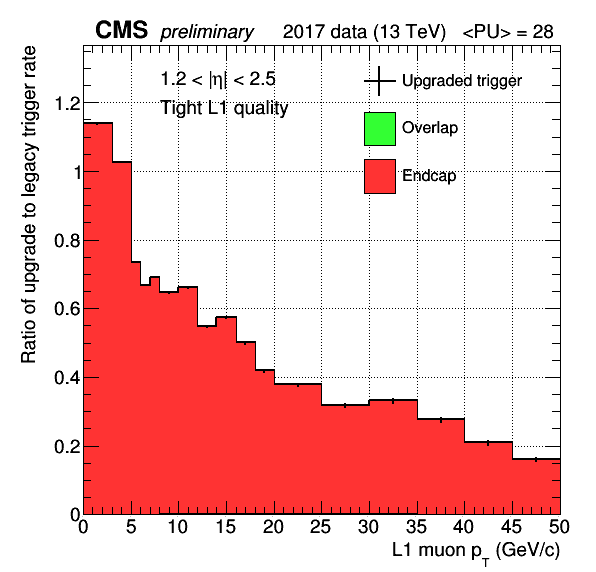
\includegraphics[width=2.5in]{images/emtf_rate_reduction.png}
  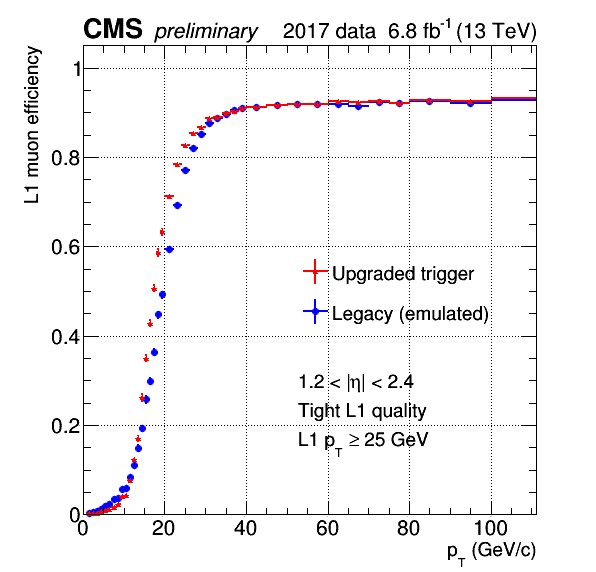
\includegraphics[width=2.5in]{images/emtf_efficiency.png}
  \caption[EMTF rate reduction and efficiency.]
   {On the left, the upgraded EMTF rate divided by the legacy rate is shown for a variety of $p_t$ thresholds. On the right, the upgraded and legacy efficiencies are presented for a 25 GeV threshold. The upgraded EMTF has a 3x lower rate than the legacy system at 25 GeV with virtually no difference in plateau efficiency for the same threshold. Plots are taken from \cite{CMS-DP-2017-041}.}
\label{fig:results}
\end{figure}

\section{Classifying Events}

Practically, it is difficult to perform a statistical analysis with a PDF in many dimensions. In a binned analysis, the density of the data points in each bin decays rapidly as the number of dimensions increase. To mitigate this problem, the $H\rightarrow\mu^+\mu^-$ analysis uses a one dimensional PDF along the dimuon mass spectrum. Unforunately, collapsing the muon and jet information mixes areas of high sensitivity with areas of low sensitivty and undercuts the power for discovery. To recover the lost sensitivity, the analysis uses the muon and jet information in the MC to train Boosted Decision Trees (BDTs) to distinguish signal from background. The BDTs map the events from the many kinematic dimensions onto the BDT score, whose spectrum places a large density of signal and low density of background at large values.  

The high BDT score regions will have $m_{\mu\mu}$ distributions with more signal in the peak over less background, recovering the sensitivity. The sensitivity can be further improved by concentrating the signal peak into a narrower region. To this end, the events are extracted and placed into categories based upon both the BDT score and the mass resolution.     

\subsection{Training Boosted Decision Trees}

BDTs are trained using ROOT's TMVA to distinguish signal from the major backgrounds, Drell-Yan (DY) and $t\bar{t}$. VBF is easiest to distinguish from Drell-Yan as the VBF channel has two jets at leading order, while Drell-Yan has none. VBF events characteristically have two forward jets with large dijet mass. A top quark decays most often to a W and b, and to be seen in $\mu^+\mu^-$ data the W decays to a neutrino and a muon. As a result, the $t\bar{t}$ events may be distinguished by the presence of b-jets and above average MET. GGF and DY are very similar. In GGF, two gluons fuse and make a Higgs, which then decays to two muons. In DY, two quarks fuse and make a Z/photon which then decays to two muons.  In both cases, the final state at leading order is just the two muons. However, gluons are a bit more likely to radiate jets than quarks, so the average dimuon $p_t$ is a bit higher for GGF. The dimuon $p_t$ provides some discrimination power as do the jet variables, but the GGF and DY events are still very similar on average.  

The features used to train the BDTs are chosen to maximize the discrimination capabilities without changing the $m_\mu\mu$ distribution. The features are
\begin{itemize}
\item the $p_t$ and $\eta$ of the dimuon system, \vspace{-10pt}
\item the $|\Delta\eta|$ and $|\Delta\phi|$ between the muons, \vspace{-10pt}
\item the $\eta$ values of the two highest--$p_t$ jets, \vspace{-10pt}
\item the masses of the two highest--mass dijet pairs, \vspace{-10pt}
\item the $|\Delta\eta|$ bewteen the jets in the two highest--mass pairs, \vspace{-10pt}
\item the number of jets with $|\eta| < 2.4$ and $|\eta| > 2.4$, \vspace{-10pt}
\item the number of jets passing the CSVv2 medium b-tag working point, \vspace{-10pt}
\item and the MET.
\end{itemize}
The $p_t$ for the individual muons is left out to prevent any reshaping of $m_{\mu\mu}$. If any peaks or troughs are arbitrarily created in the $m_{\mu\mu}$ spectrum, this could lead to a false discovery. The feature importance at first order is listed in Table \ref{tab:featureranking}. The ranking plots histograms of the signal and background along the feature and finds the percentage of the total area that does not overlap.
\begin{table}[htb]
  \caption[The feature importance.]{The importance is given by the percentage of the signal and background PDFs along that feature that do not overlap.}
  \label{tab:featureranking}
  \begin{center}
    \begin{tabular}{lr}
      \hline
      Feature  & Importance \\
      \hline
      Dimuon $p_t$               &    5.342e-02    \\
      Dimuon $\eta$              &    3.896e-02    \\
      $|\delta\phi(\mu\mu)|$     &    3.500e-02    \\
      Number of medium b-tags    &    2.842e-02    \\
      $\eta(jet1)$               &    1.724e-02    \\
      MET                        &    1.706e-02    \\
      Number of forward jets     &    1.218e-02    \\
      $|\delta\eta(jj_{1})|$     &    8.310e-03    \\
      Number of central jets     &    8.036e-03    \\
      $\eta(jet2)$               &    7.460e-03    \\
      $|\delta\eta(\mu\mu)|$     &    6.793e-03    \\
      $M(jj_{1})$                &    6.546e-03    \\
      $|\delta\eta(jj_{2})|$     &    3.304e-03    \\
      $M(jj_{2})$                &    2.199e-03    \\
      \hline
    \end{tabular}
  \end{center}
\end{table}

The BDT training and optimization uses 50\% of the available DY and $t\bar{t}$ MC for training and $50\%$ to evaluate the effectiveness of the training. On the other hand, 25\% of the major signal MC (GGF, VBF, and VH) is used for training and 25\% for testing, and 50\% is excluded from training/evaluation. The excluded 50\% of the signal MC is used at a later stage for an unbiased report of the limits. The background PDF used for the limits is estimated from the sidebands in the data, so it's not necessary to withold any of the background MC. The number of trees, nodes, and learning rate were optimized based upon the area under the Receiver Operating Characteristic (ROC) curve. The final BDT settings use 500 trees, a depth of 5, and a learning rate of 0.1. The gradient boosting optimizes the binary cross entropy loss function. 

Histograms over the features are shown in Figures \ref{fig:valid_bdt_incl-a} and \ref{fig:valid_bdt_incl-b} for the events passing the initial event selection. The separation of the signal and background along the BDT score is plotted in Figure \ref{fig:bdt_score_inclusive}. The Receiver Operating Characteristic (ROC) curve for the final BDT model is shown in Figure \ref{fig:BDT_ROC}. With the BDT score the events may now be categorized. 
\begin{figure}[h!]
  \includegraphics[width=0.5\linewidth]{images/bdt_training/BDT_ROC_ge0j_all.pdf}
  \caption[The BDT ROC score for signal vs background classification.]
  {The background-rejection vs. signal efficiency ROC curve for the final BDT model.} 
  \label{fig:BDT_ROC}
\end{figure}

\FloatBarrier
\subsection{Event Categorization}
\label{bdt_cats}

The analysis optimizes the sensitivity of the $H\rightarrow \mu^+\mu^-$ search, by categorizing the events
based on two criteria: the BDT output score and the muon $|\eta|$ information.
The output score of the BDT is used to separate signal
from background events, where the score ranges from -1 (background-like) to +1 (signal-like).
The maximum $|\eta|$ value of the two candidate muons is used to select events with better mass resolution. 
In order to optimize the choice of BDT and $|\eta|$ cuts, the analysis designed and implemented
a decision tree autocategorizer to create categories by greedily optimizing a metric corresponding
to the sensitivity. The BDT training and the autocategorization
are performed on 50\% of the signal MC events and 100\% of the background MC events. The autocategorizer uses the same background and signal MC as the BDT training.
After training the autocategorizer on the signal and background MC to determine the categories,
the expected limits are calculated using data and the remaining 50\% of simulated signal events. Separating the
signal MC into exclusive sets for optimization and limit evaluation, and excluding the data from the training phase, ensure an unbiased estimate for the limits.

\begin{figure}[h!]
  \centering
  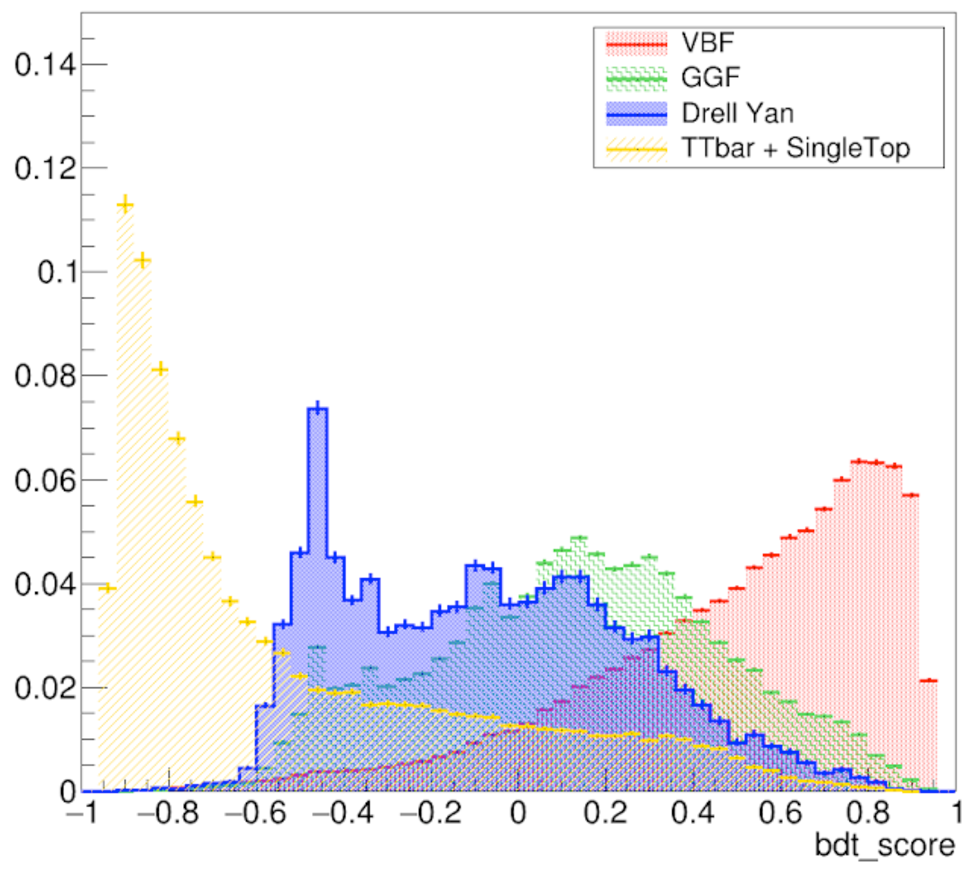
\includegraphics[width=0.49\linewidth]{images/bdt_cats/bdt_score_ggH_VBF_DY_ttbar.pdf}
  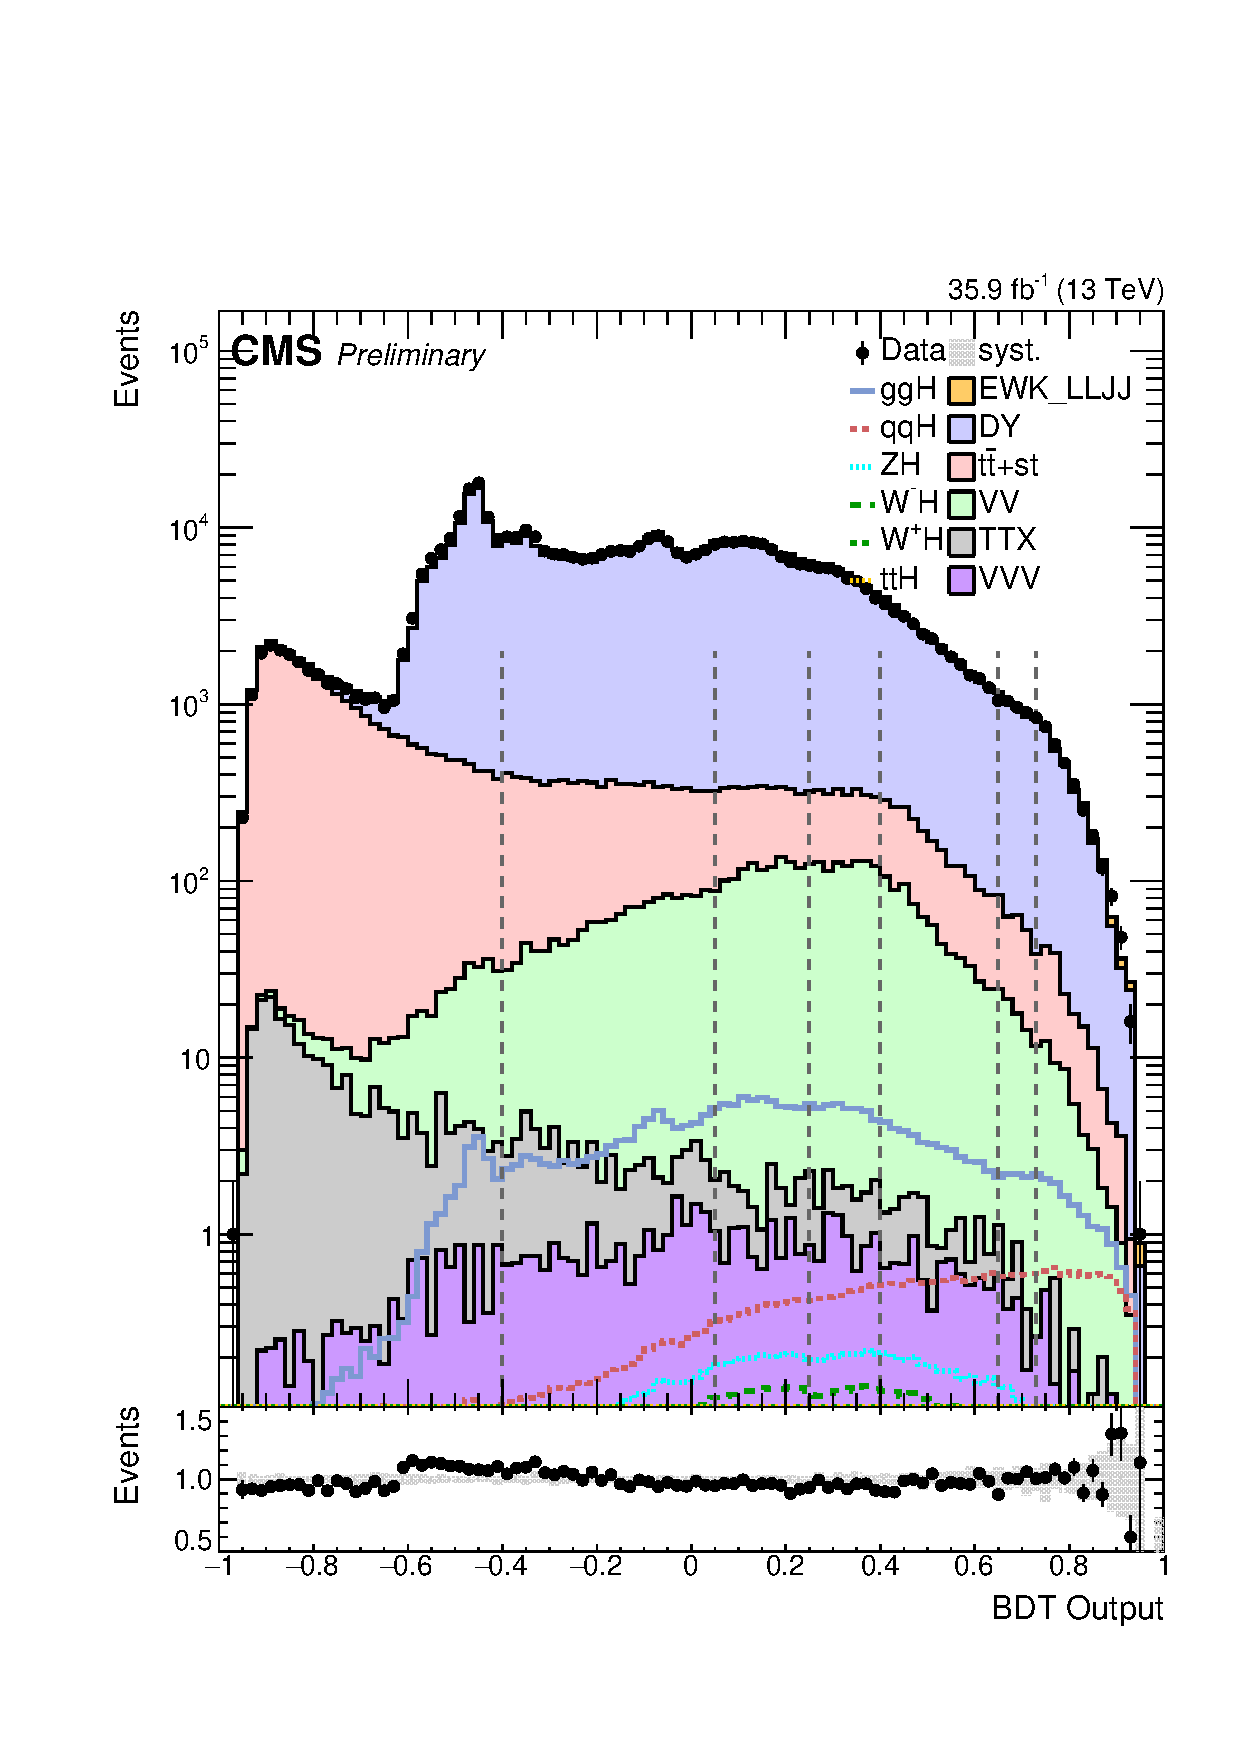
\includegraphics[width=0.49\linewidth]{images/bdt_cats/BdtOnH_bkg.pdf}
 %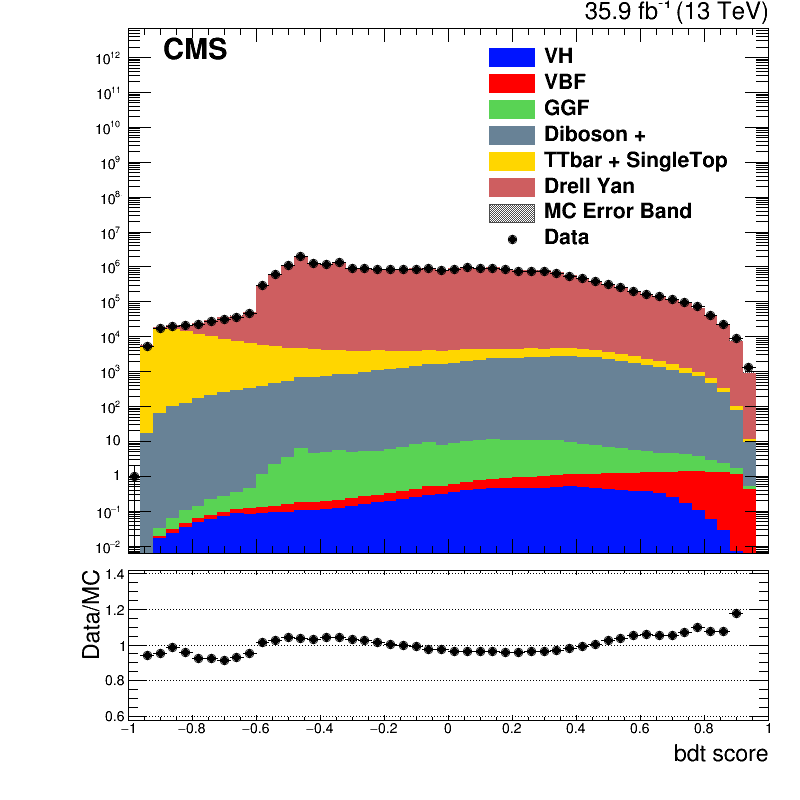
\includegraphics[width=0.49\linewidth]{images/bdt_cats/bdt_score_cAll.png}
  \caption[BDT score distributions for signal MC, background MC, and data.]
   {The BDT score on the signal and background Monte Carlo (left). A higher score indicates signal-like events.
    Note $t\bar{t}$ on the left as the most distinguishable background and VBF on the right as the most distinguishable signal.
    The BDT score in data is modeled well by the amc@NLO Drell--Yan MC (right).}
  \label{fig:bdt_score_inclusive}
\end{figure}

\FloatBarrier
\subsection{The Autocategorizer}

A novel algorithm has been designed to categorize the events and maximize the sensitivity of the search.
The categorization takes into account both the signal/background discrimination and the resolution of the mass peak.
In order to account for the resolution, the signal and background events are binned in half-GeV bins in the signal
region of the dimuon mass spectrum, 120 to 130 GeV. 
\begin{figure}[h!]
  \centering
  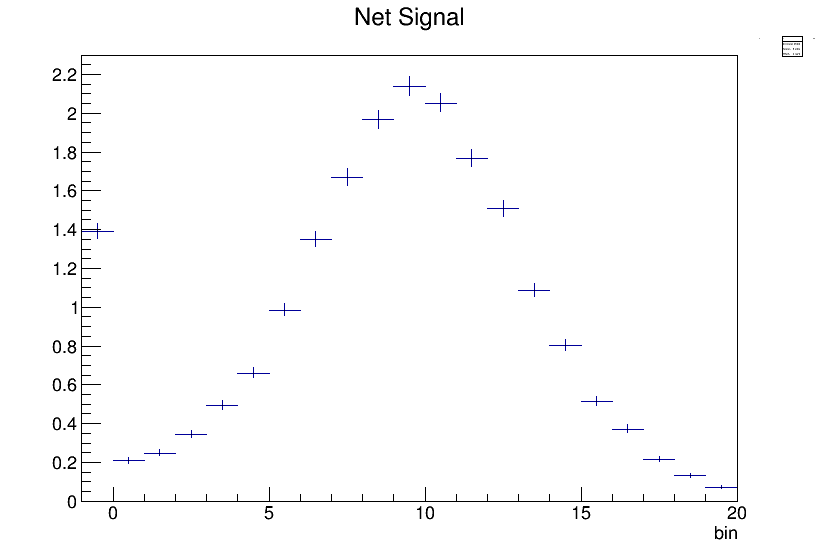
\includegraphics[width=0.49\linewidth]{images/bdt_cats/binning_signal_example.png}
  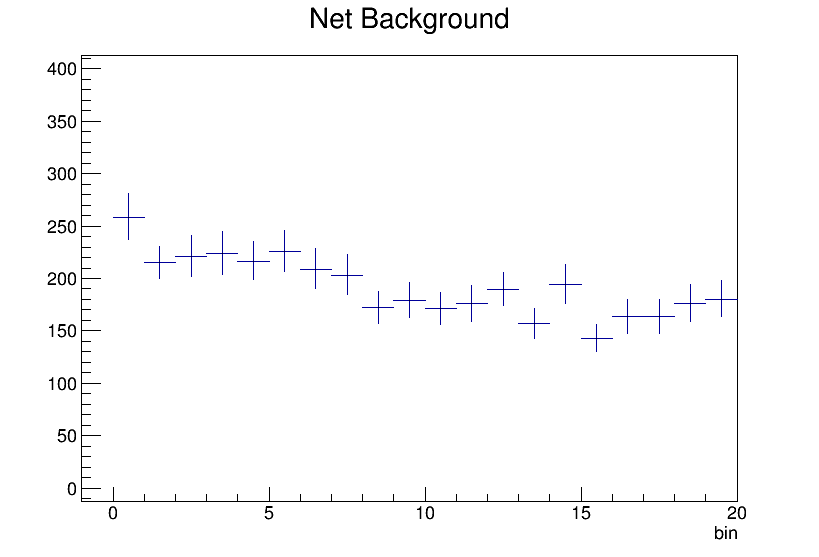
\includegraphics[width=0.49\linewidth]{images/bdt_cats/binning_bg_example.png}
  \caption[An example of the signal and background histograms for the Autocategorizer.]
  {An example of the binned signal and background necessary for the significance metric. The binning keeps the most sensitive bins
   from being drowned out by the others, providing a measure that accounts for both signal--background discrimination and resolution.}
  \label{fig:binning_example}
\end{figure}
The significance in each bin is then given by $S/\sqrt{B}$.
The significance for independent bins adds in quadrature, so the net significance is given by
\begin{equation}
{\rm Net~Significance} = \sum_{c,i}S_{c,i}^{2}/B_{c,i}
\end{equation}
where $i$ labels the bin in the signal region, and $c$ denotes the category. $S_{c,i}$ is the number of expected signal
events in the $i^{th}$ bin in that category, and $B_{i,c}$ is the number of expected background events in the $i^{th}$ bin.
By binning finely enough, the central mass bins contribute the most and the resolution is accounted for.

On the first iteration, the autocategorizer calculates the net significance for the set of all events, the inclusive set.
The algorithm then searches over the inclusive set, checking all possible split values of the maximum muon $|\eta|$. Events
with maximum $|\eta|$ values less than the split go in one candidate category, and those with max $|\eta|$ values greater than or equal
to the split value go into the other candidate category. For every split candidate, the algorithm calculates the net significance
in the two categories delineated by the split value. The maximum $|\eta|$ cut value that provides the largest gain in significance
over the inclusive set is stored. The gain is defined in the equation below where $c1$ and $c2$ are the prospective categories
created from $c$ by splitting on the feature.
\begin{equation}
{\rm Gain} = \sum_{i}S_{c1,i}^{2}/B_{c1,i} + \sum_{i}S_{c2,i}^{2}/B_{c1,i} - \sum_{i}S_{c,i}^{2}/B_{c,i} 
\end{equation}
The autocategorizer then searches over the BDT score values and stores the BDT score that provides the largest gain in significance.
The algorithm chooses to split on either the maximum muon $|\eta|$ or the BDT score (whichever has the higher gain), creating two
categories from the inclusive set of events. At the next iteration, the autocategorizer repeats the procedure for the two new
categories and chooses to split the category that provides the most gain. This process continues, each time greedily choosing to
split the category with the most gain, until the number of categories desired is reached.


\begin{figure}[h!]
  \centering
  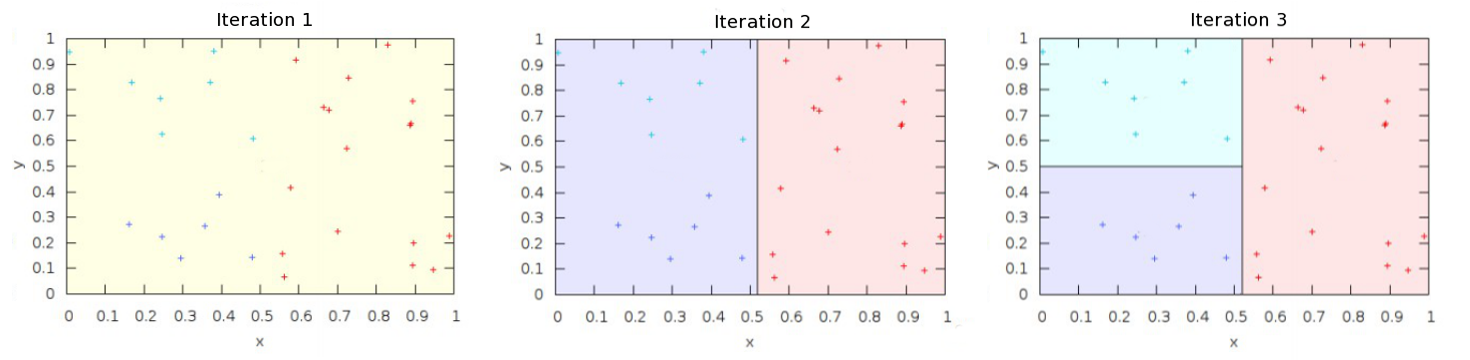
\includegraphics[width=0.98\linewidth]{images/bdt_cats/iter_all.png}
  \caption[An example of the autocategorization process.]
  {An example of the categorization process for some toy features x and y and three categories. The colored crosses represent the events that should be grouped together for optimum sensitivity. After three iterations, the categorizer correctly groups those events. The autocategorizer chooses x=0.52 for the first split and y=0.50 for the second.}
  \label{fig:iter_example}
\end{figure}

\FloatBarrier
\subsection{Final Categories}

After training the BDT and autocategorizing based upon the maximum muon $|\eta|$ and the BDT score, the resulting categorization is
formed by rounding some of the cuts. Care is taken so that the simplification does not worsen the
expected limit. 
\begin{figure}[h!]
  \centering
  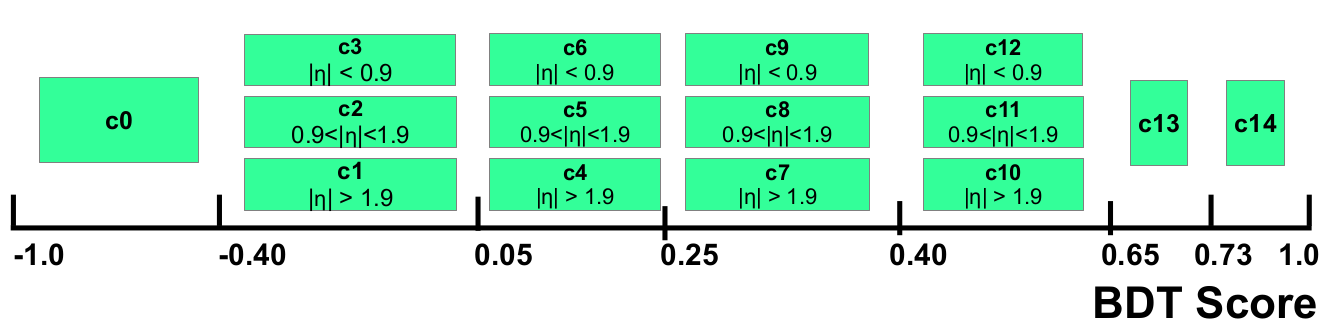
\includegraphics[width=1.0\linewidth]{images/bdt_cats/final_categories_symb-eta.png}
  \caption[The final categorization.]
   {The final categorization.}
  \label{fig:final_categories}
\end{figure}
The 15 BDT categories produced by the Autocategorizer in Figure~\ref{fig:final_categories}
show a 23\% improvement compared to the 15 Run~I $H\rightarrow\mu^+\mu^-$ categories.
For the comparison, the expected upper limits are evaluated on the same 36 $fb^{-1}$ of 2016 data and signal Monte Carlo in the
same way for an even comparison. The categories are ordered by BDT Score and $|\eta|$.

The FWHM of the mass resolution, the expected signal and background
yields, the sensitivity, and the expected limit for each of the final 15 categories are
shown in Table~\ref{tab:cat_resoln}.

\begin{table}[htb]
  \caption[The characteristics of each category.]
           {Full Width Half Max (FWHM) of the signal peak, expected signal and background yields within the FWHM,
           purity, sensitivity, and the expected upper limits at 95\% confidence. 
           The background yields and the expected limits use background models fit to the data in the sidebands.}
  \label{tab:cat_resoln}
  \begin{center}
    \begin{tabular}{crrrrrr}
      \hline
      Category  & Signal FWHM (GeV) & Signal & Background & $\mathrm{S / B}$ (\%) & $\mathrm{S / \sqrt{B}}$ & Limit \\  %% & Signal events
      \hline
        c0         &         4.4     &        13.3     &        14400    &        0.000927    &     0.111    &  19    \\
        c1         &         6.0     &        13.9     &        7990     &        0.00174     &     0.156    &  16    \\
        c2         &         4.3     &        27.7     &        10000    &        0.00276     &     0.277    &  7.9   \\
        c3         &         3.1     &        8.70     &        2600     &        0.00334     &     0.170    &  12    \\
        c4         &         6.3     &        7.66     &        2750     &        0.00279     &     0.146    &  17    \\
        c5         &         4.3     &        19.6     &        4320     &        0.00453     &     0.298    &  7.1   \\
        c6         &         3.1     &        9.86     &        1540     &        0.00638     &     0.250    &  8.4   \\
        c7         &         6.2     &        3.44     &        928      &        0.00370     &     0.113    &  22    \\
        c8         &         4.3     &        14.0     &        2310     &        0.00607     &     0.292    &  7.9   \\
        c9         &         3.2     &        8.85     &        1050     &        0.00838     &     0.272    &  7.3   \\
        c10        &         6.2     &        3.62     &        641      &        0.00564     &     0.142    &  16    \\
        c11        &         4.5     &        14.4     &        1830     &        0.00788     &     0.338    &  6.1   \\
        c12        &         3.4     &        10.1     &        855      &        0.0118      &     0.348    &  6.1   \\
        c13        &         4.2     &        6.15     &        422      &        0.0145      &     0.299    &  7.7   \\
        c14        &         4.5     &        9.84     &        387      &        0.0254      &     0.500    &  4.6   \\
      \hline
    \end{tabular}
  \end{center}
\end{table}

\FloatBarrier
\subsection{Validating The Categories}

It is important that the signal is correctly modeled in each category in order to report an accurate expected upper limit.
Figures \ref{fig:valid_bdt_incl-a} and \ref{fig:valid_bdt_incl-b} show the data/MC agreement for the BDT features as well as the dimuon mass
for the inclusive set of events with dimuon mass greater than 60~GeV.

\begin{figure}[h!]
  \centering
  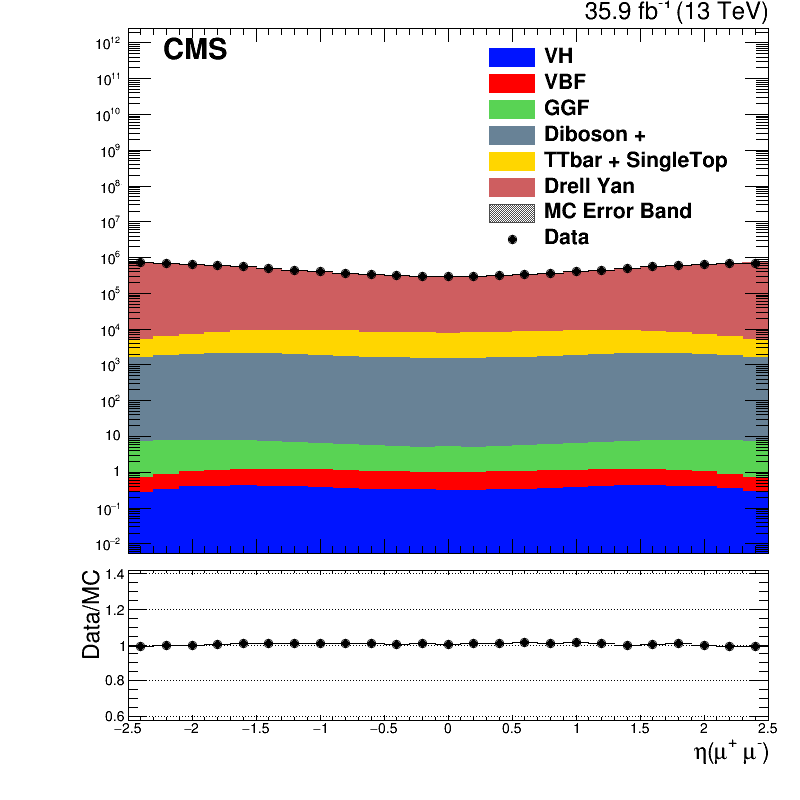
\includegraphics[width=0.32\linewidth]{images/bdt_cats/dimu_eta_cAll.png}
  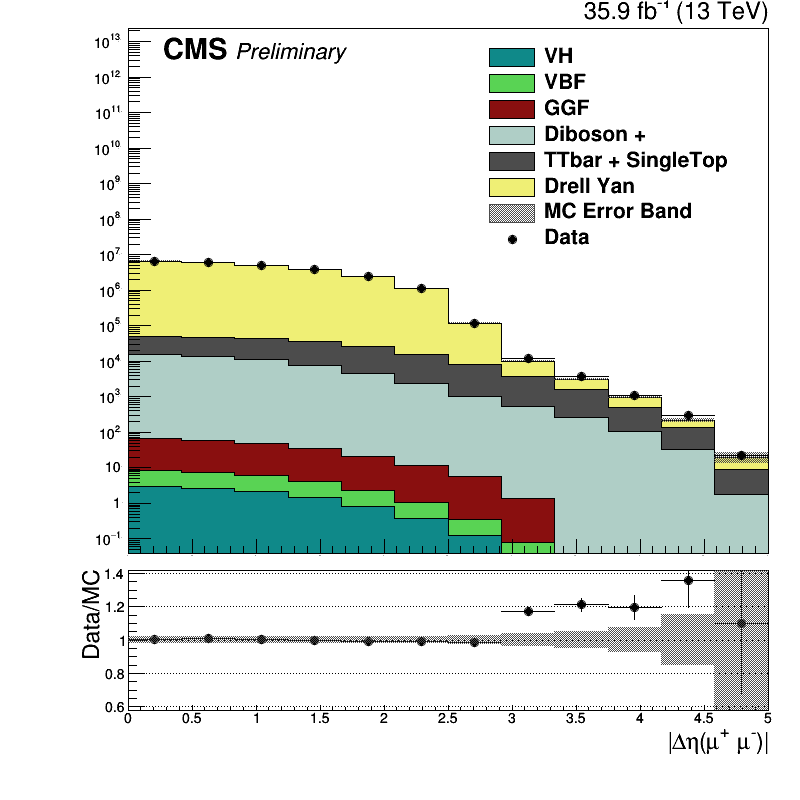
\includegraphics[width=0.32\linewidth]{images/bdt_cats/dimu_abs_dEta_cAll.png}
  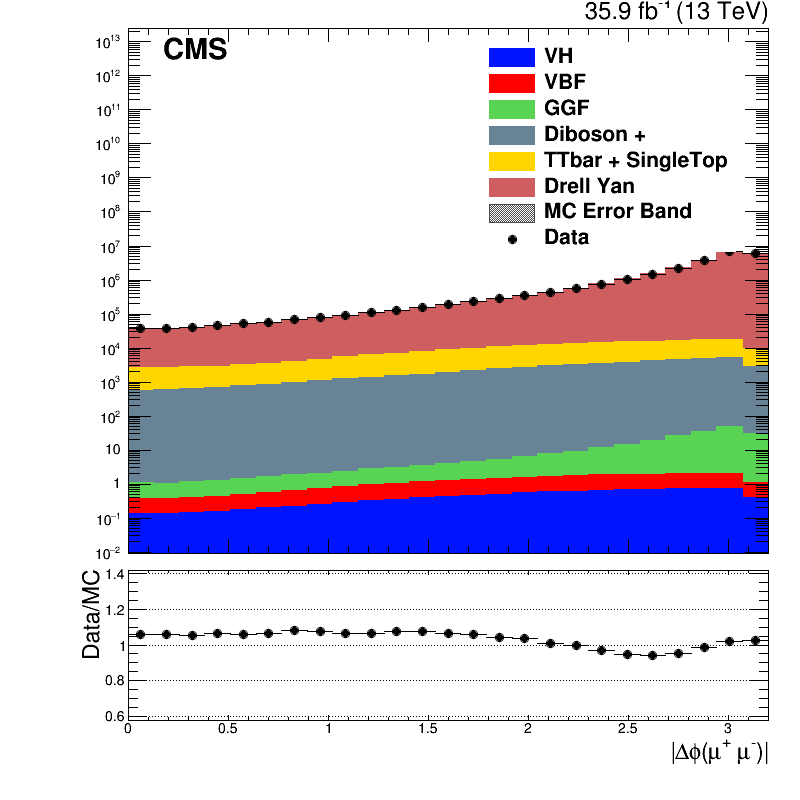
\includegraphics[width=0.32\linewidth]{images/bdt_cats/dimu_abs_dPhi_cAll.png}
  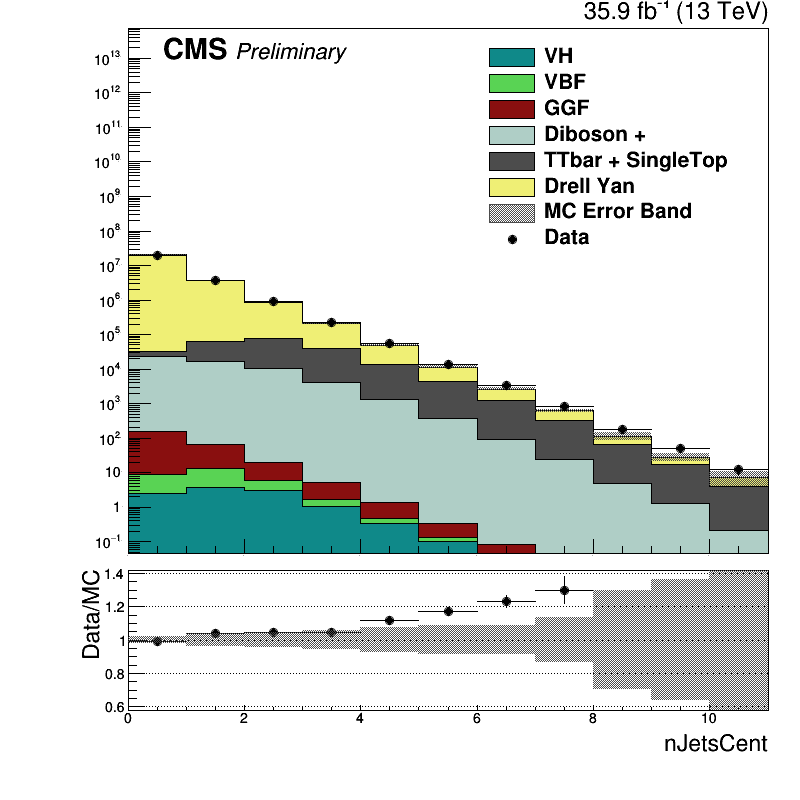
\includegraphics[width=0.32\linewidth]{images/bdt_cats/nJetsCent_cAll.png}
  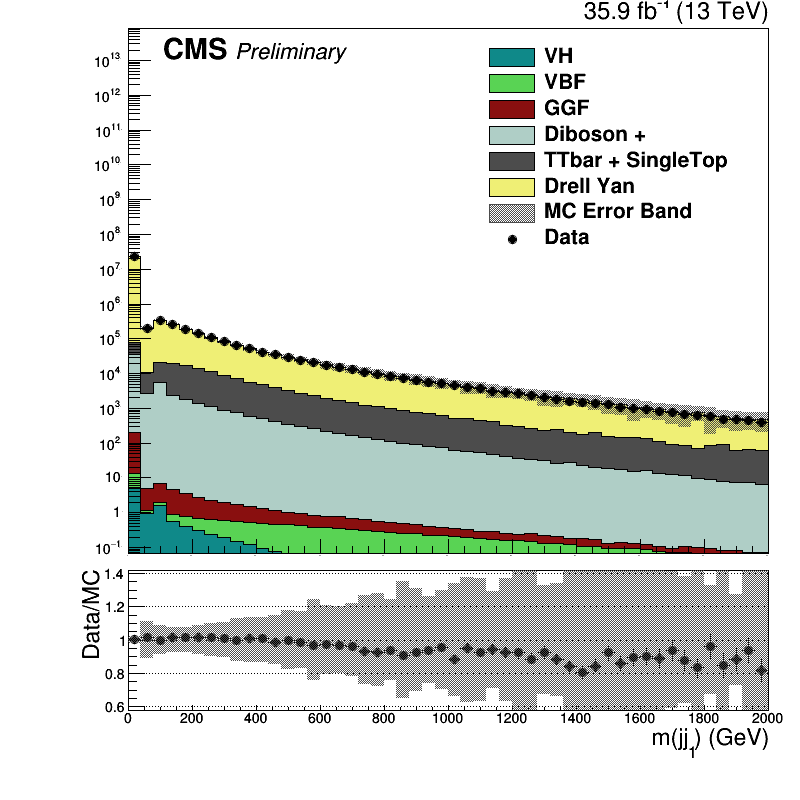
\includegraphics[width=0.32\linewidth]{images/bdt_cats/dijet1_mass_cAll.png}
  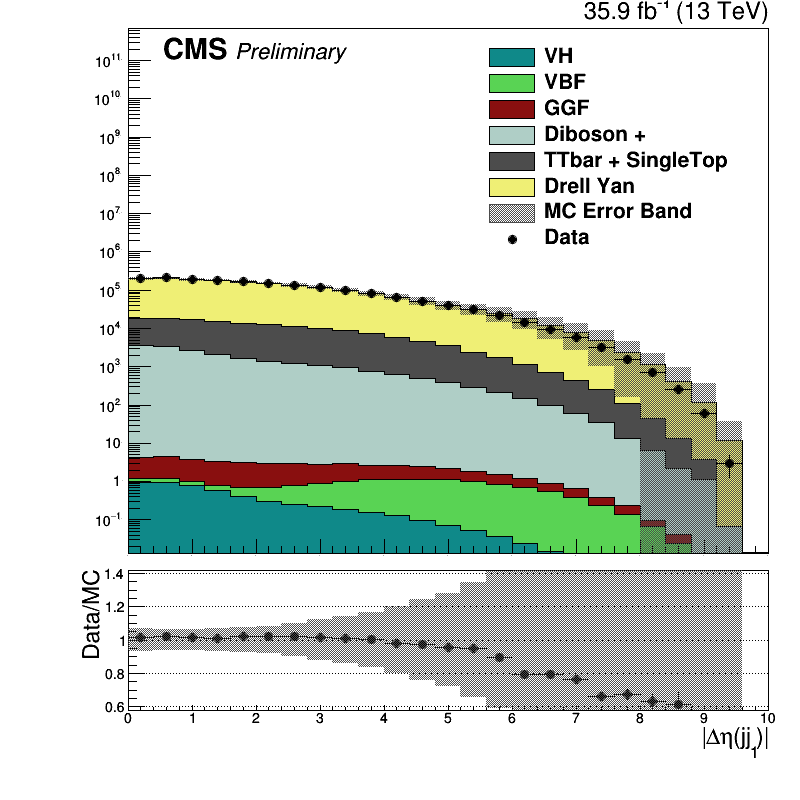
\includegraphics[width=0.32\linewidth]{images/bdt_cats/dijet1_abs_dEta_cAll.png}
  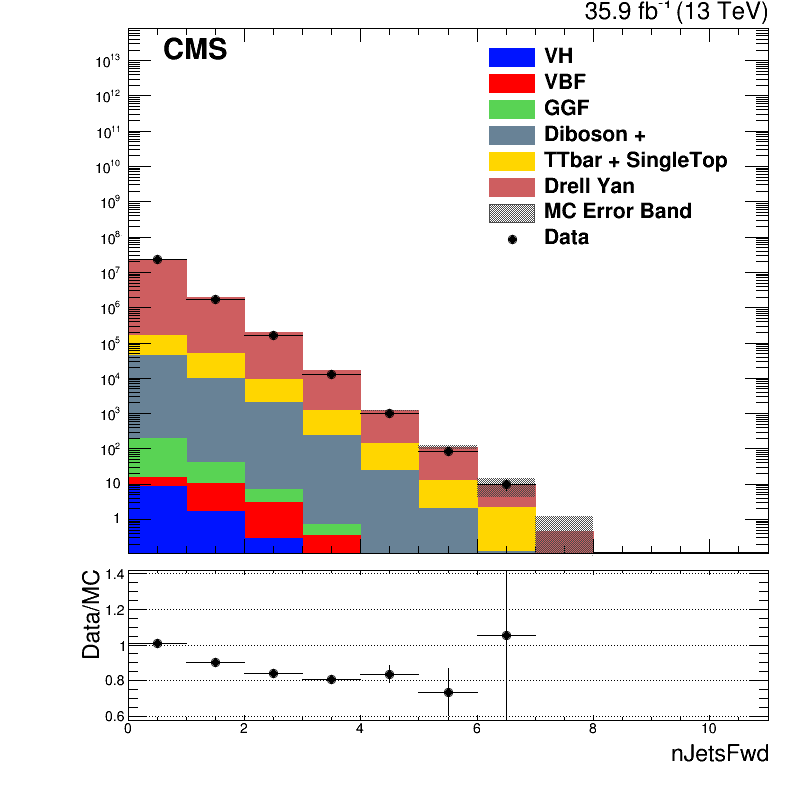
\includegraphics[width=0.32\linewidth]{images/bdt_cats/nJetsFwd_cAll.png}
  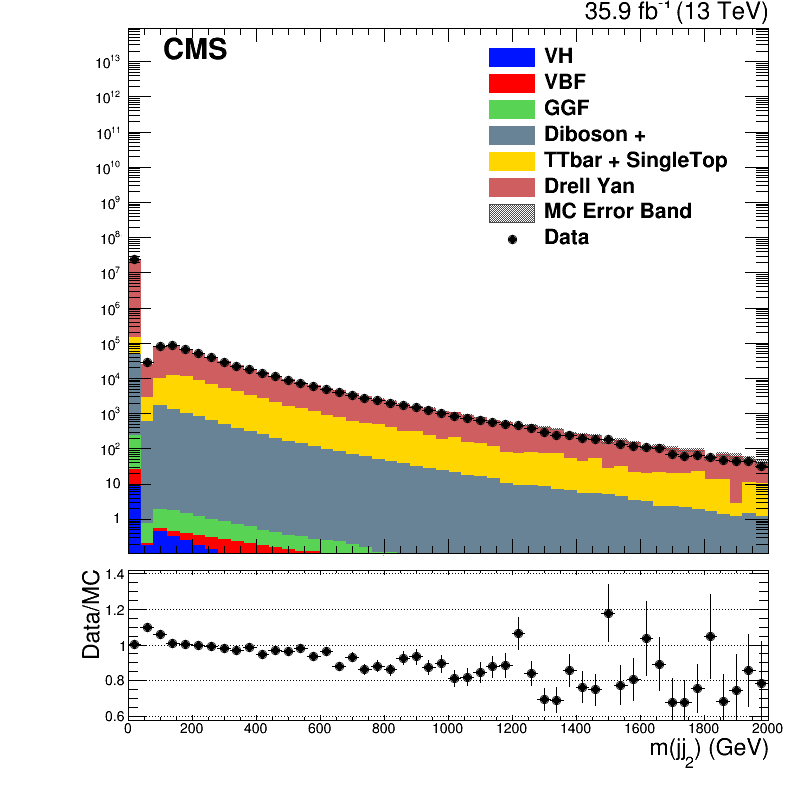
\includegraphics[width=0.32\linewidth]{images/bdt_cats/dijet2_mass_cAll.png}
  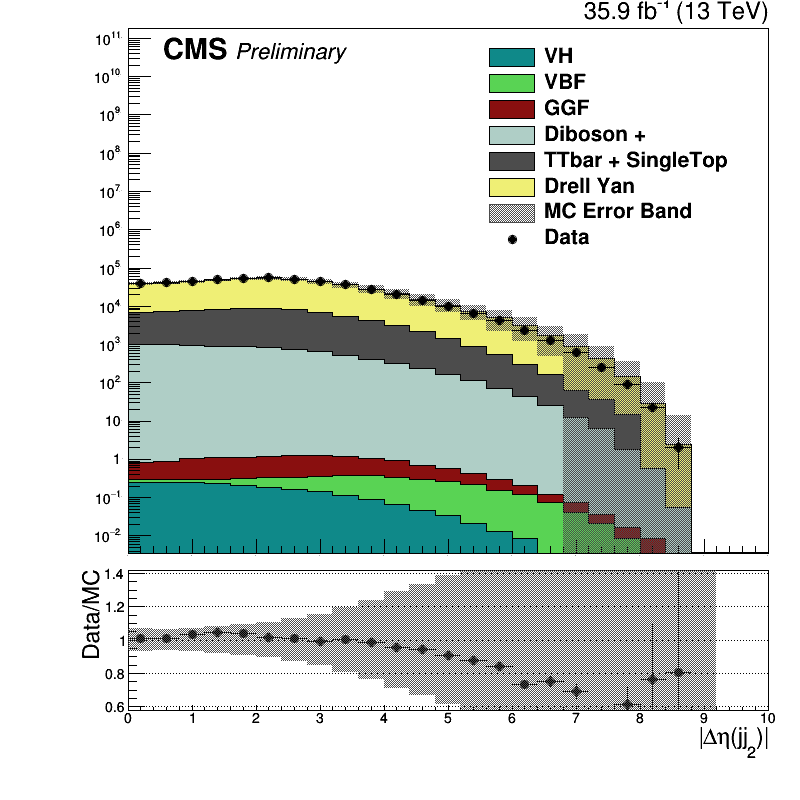
\includegraphics[width=0.32\linewidth]{images/bdt_cats/dijet2_abs_dEta_cAll.png}
  \caption[Validation plots of the BDT input variables.]
   {Validation of BDT input variables in inclusive events.}
  \label{fig:valid_bdt_incl-a}
\end{figure}

\begin{figure}[h!]
  \centering
  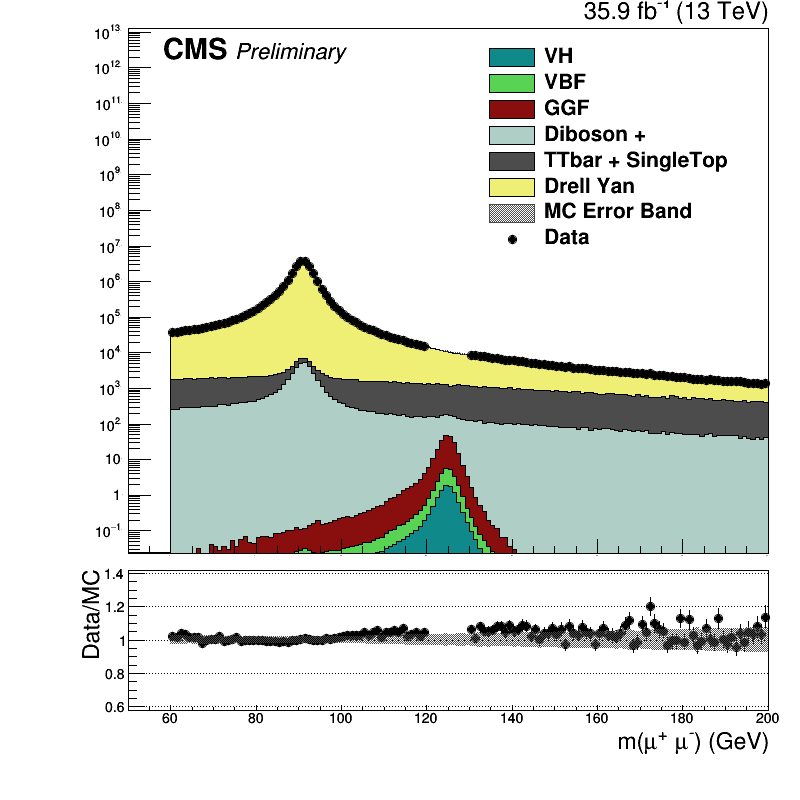
\includegraphics[width=0.32\linewidth]{images/bdt_cats/dimu_mass_Roch_cAll.png}
  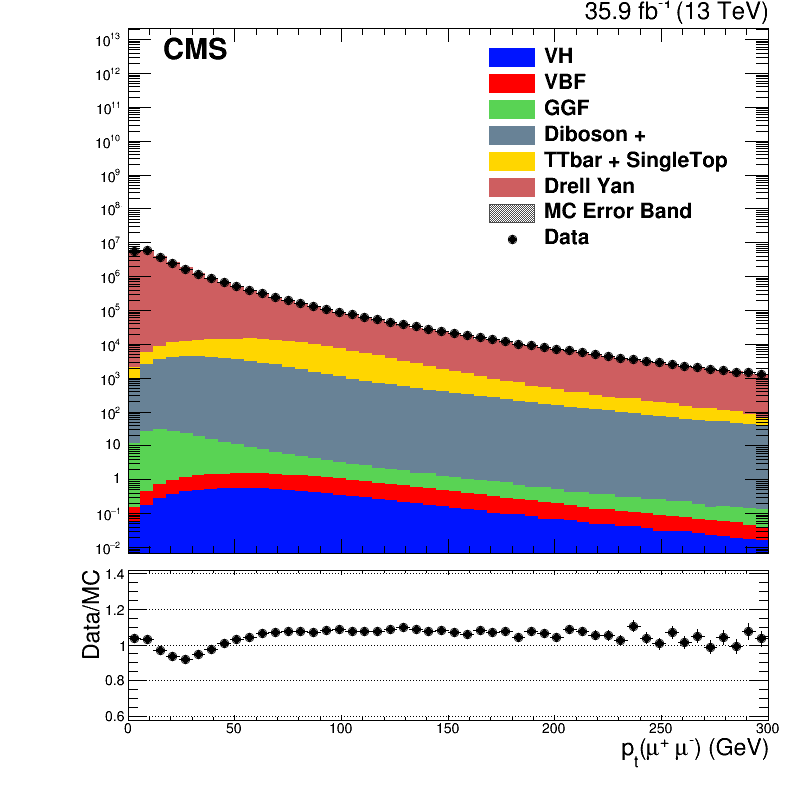
\includegraphics[width=0.32\linewidth]{images/bdt_cats/dimu_pt_cAll.png}
  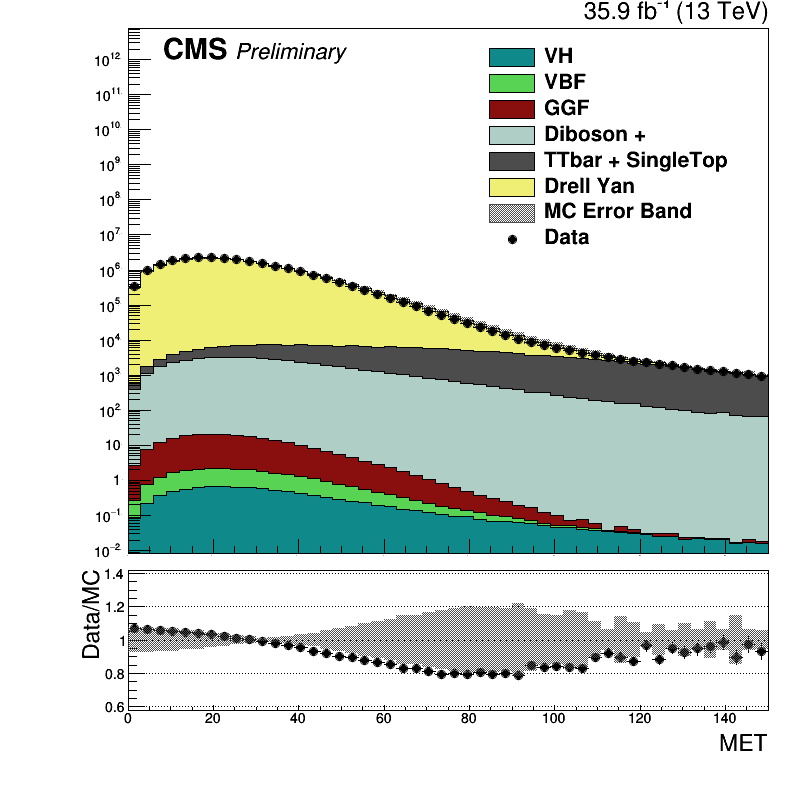
\includegraphics[width=0.32\linewidth]{images/bdt_cats/MET_cAll.png}
  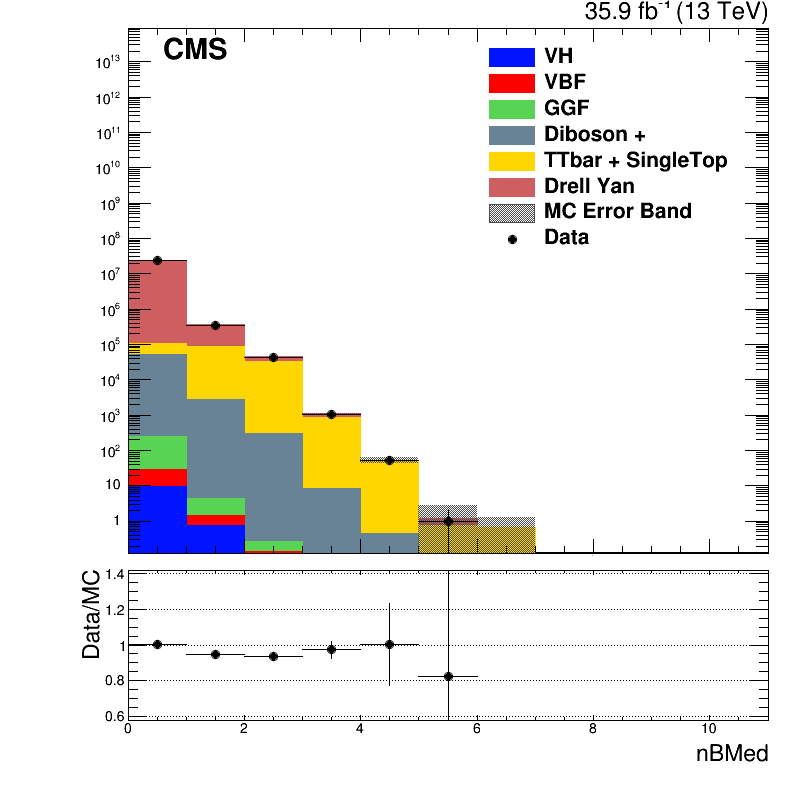
\includegraphics[width=0.32\linewidth]{images/bdt_cats/nBMed_cAll.png}
  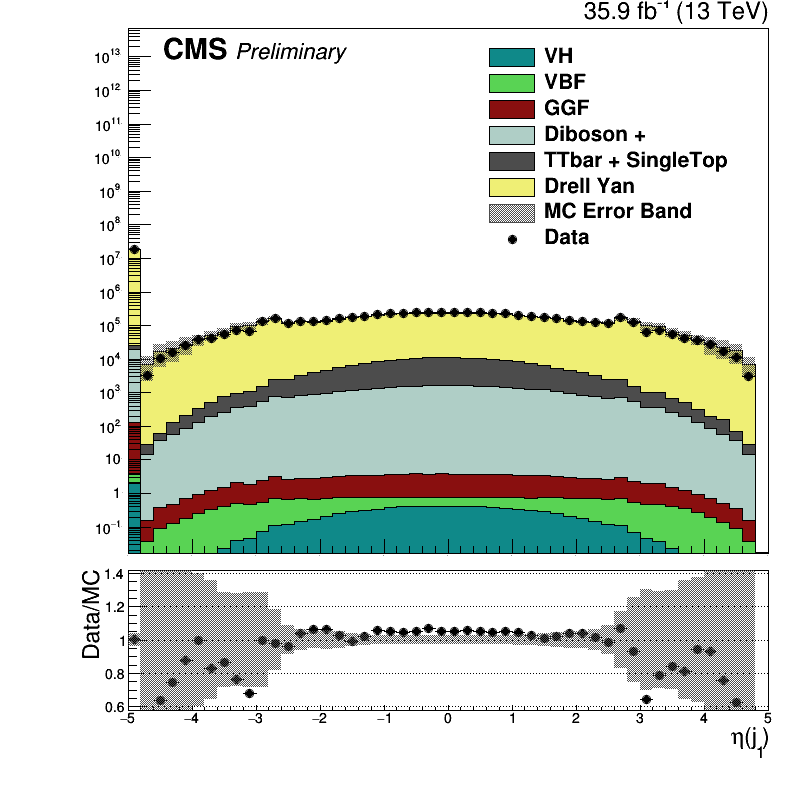
\includegraphics[width=0.32\linewidth]{images/bdt_cats/jet1_eta_cAll.png}
  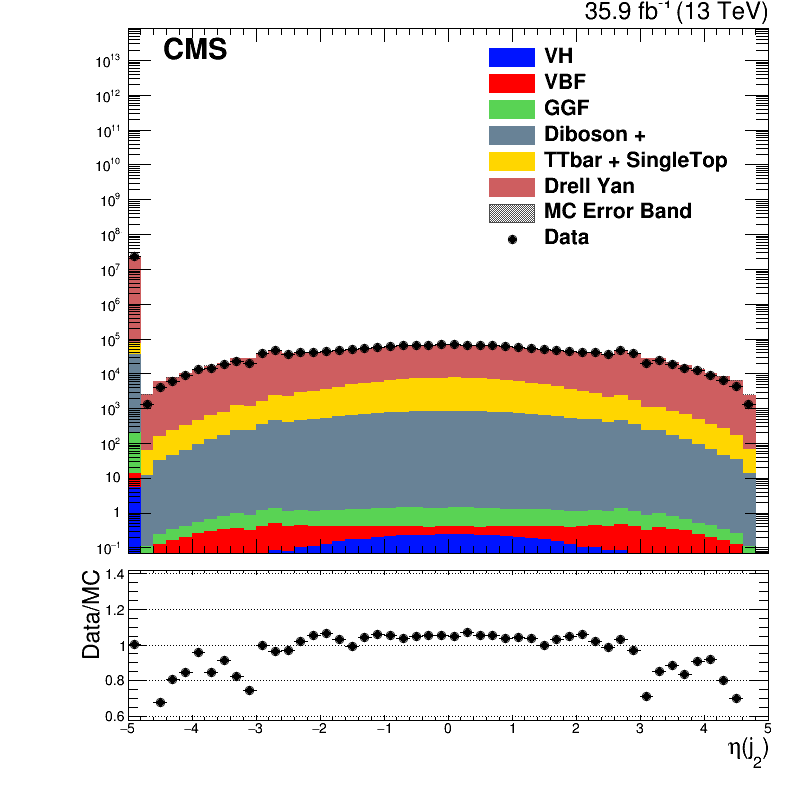
\includegraphics[width=0.32\linewidth]{images/bdt_cats/jet2_eta_cAll.png}
  \caption[Validation plots of the BDT input variables and the dimuon mass.]
   {Data/MC agreement for the inclusive events.}
  \label{fig:valid_bdt_incl-b}
\end{figure}

The Data and MC agree well. The most important variables, the BDT score, muon $\eta$, and the dimuon mass both show agreement within 10\%.
Figures~\ref{fig:valid_bdt_c14a} and~\ref{fig:valid_bdt_c14b} show the data/MC agreement for c14,
the most sensitive, most VBF-like category.
The BDT distribution in quantile is presented in Fig.~\ref{fig:bdt_quantile}
with the systematic uncertainties given by the JES and PU.
The discrepancy from -0.6 to -0.4 in the BDT score is due to the dimuon $p_t$ spectrum in Drell Yan.
The data/MC comparison of the bdt with (left) and without (right) reweighting DY dimuon $p_t$ to data
are shown in Fig.~\ref{fig:bdt_zpt}.
Note also the systematic 10\% disagreement in BDT score from -1 to -0.6 in Figure~\ref{fig:bdt_zpt} where $t\bar{t}$-like events dominate.
This region of the BDT score is defined by nBMed greater than 0 and MET greater than 40.
The 15\% disagreement in MET around 50 GeV is the largest contributor. The 10\% uncertainty
on the $t\bar{t}$ cross section may play a role as well.  Note that the disagreement takes place where the BDT score is less than $-0.4$
defining the least sensitive category. Insofar, this Data/MC discrepancy does not affect the expected limits.
Beyond the mismatch in $t\bar{t}$-like events, there is a notable Data/MC mismatch with jet $|\eta|$ $>$ 2.4, but this is expected as these are calorimeter only jets.
The disagreement in the forward jets affects high BDT score, but the discrepancy is covered by the jet energy scale and resolution uncertainties as shown in Fig.~\ref{fig:bdt_quantile}.
These uncertainties also cover the discrepancy in MET.

\begin{figure}[h!]
  \centering
  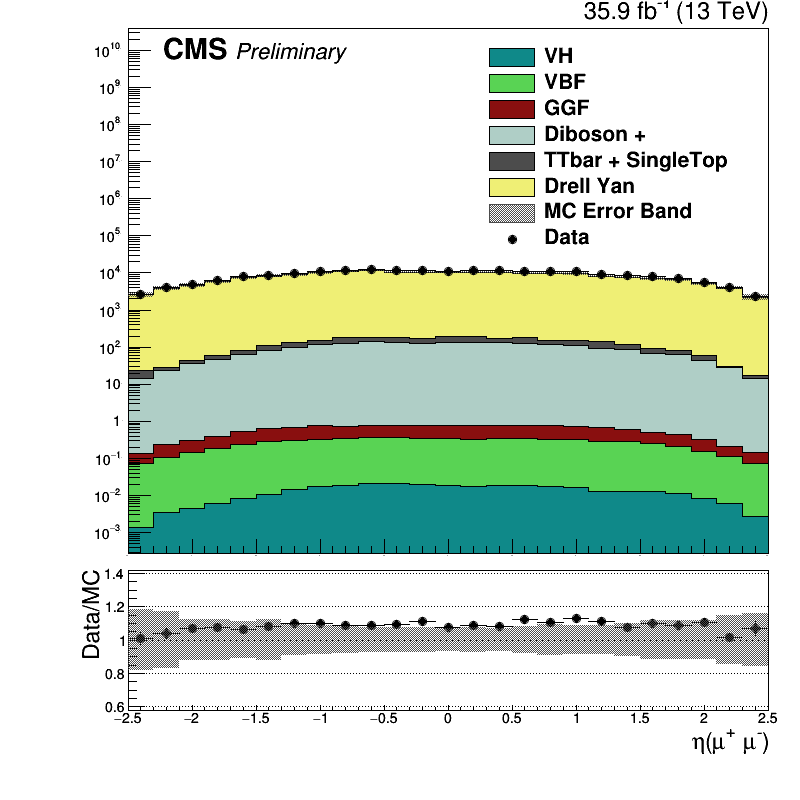
\includegraphics[width=0.32\linewidth]{images/bdt_cats/dimu_eta_c14.png}
  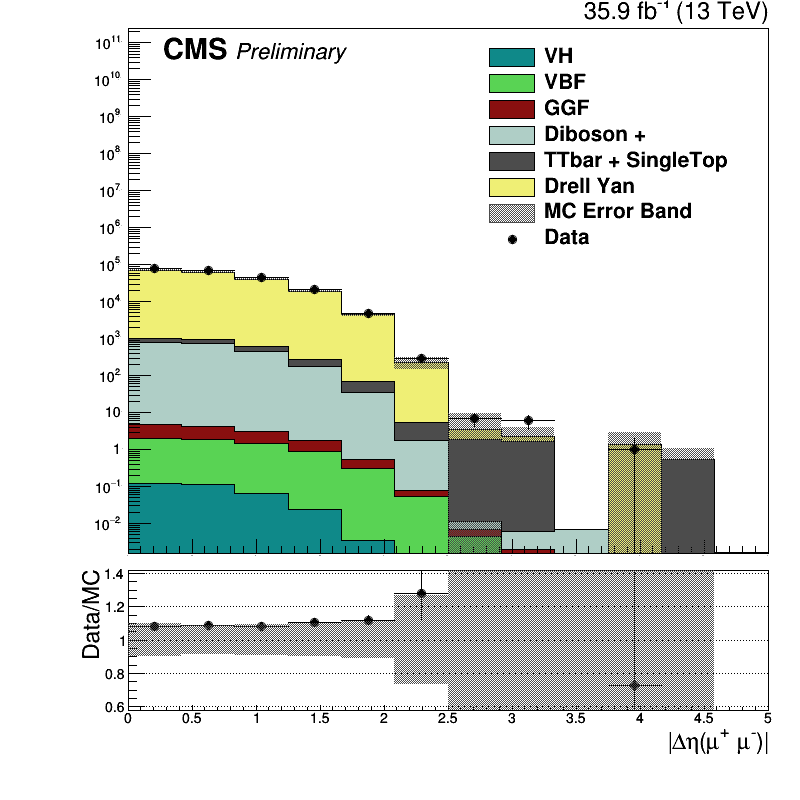
\includegraphics[width=0.32\linewidth]{images/bdt_cats/dimu_abs_dEta_c14.png}
  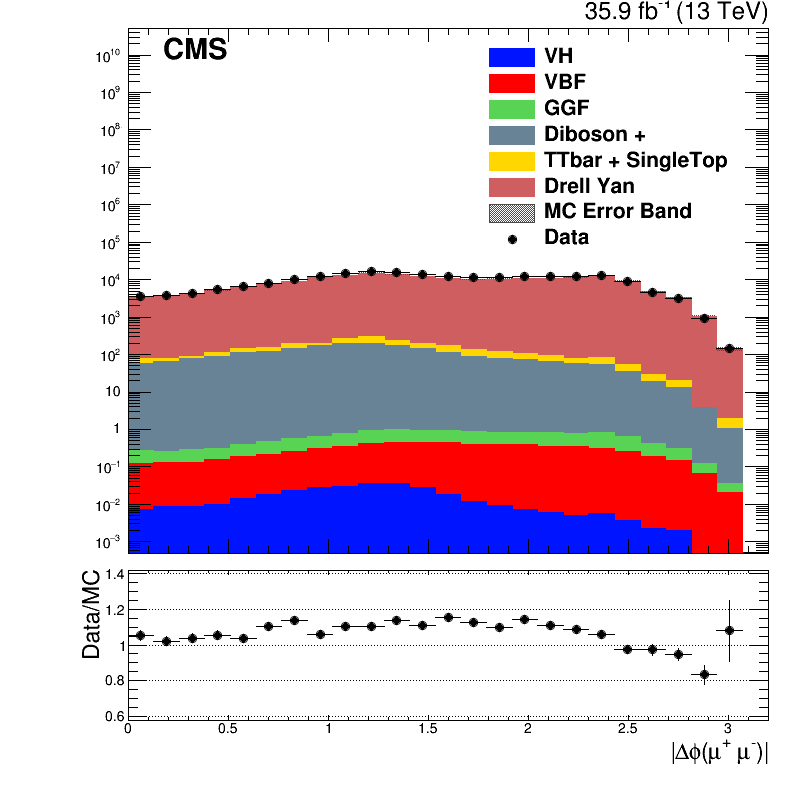
\includegraphics[width=0.32\linewidth]{images/bdt_cats/dimu_abs_dPhi_c14.png}
  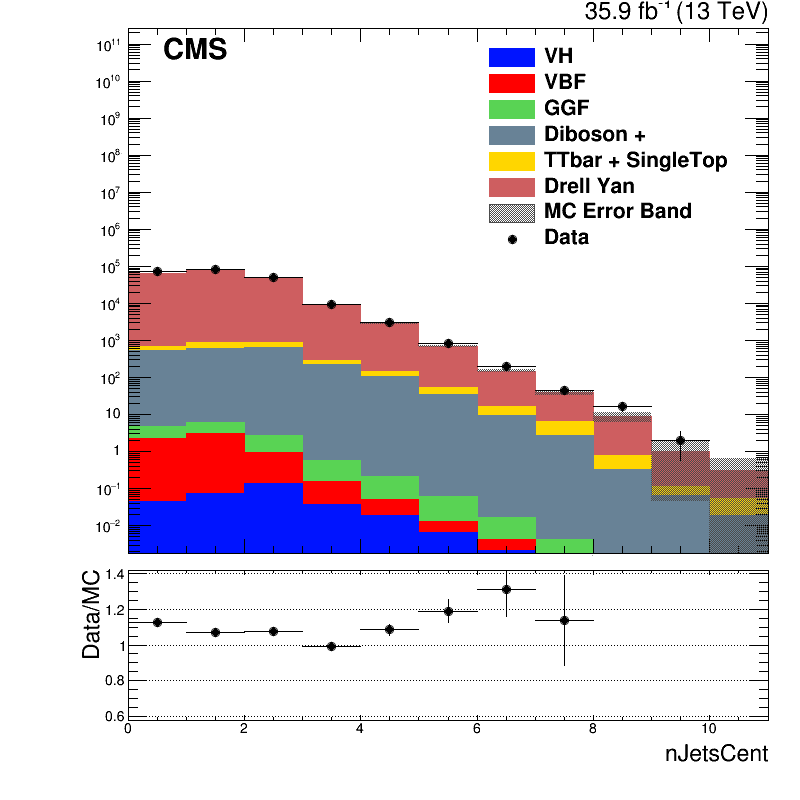
\includegraphics[width=0.32\linewidth]{images/bdt_cats/nJetsCent_c14.png}
  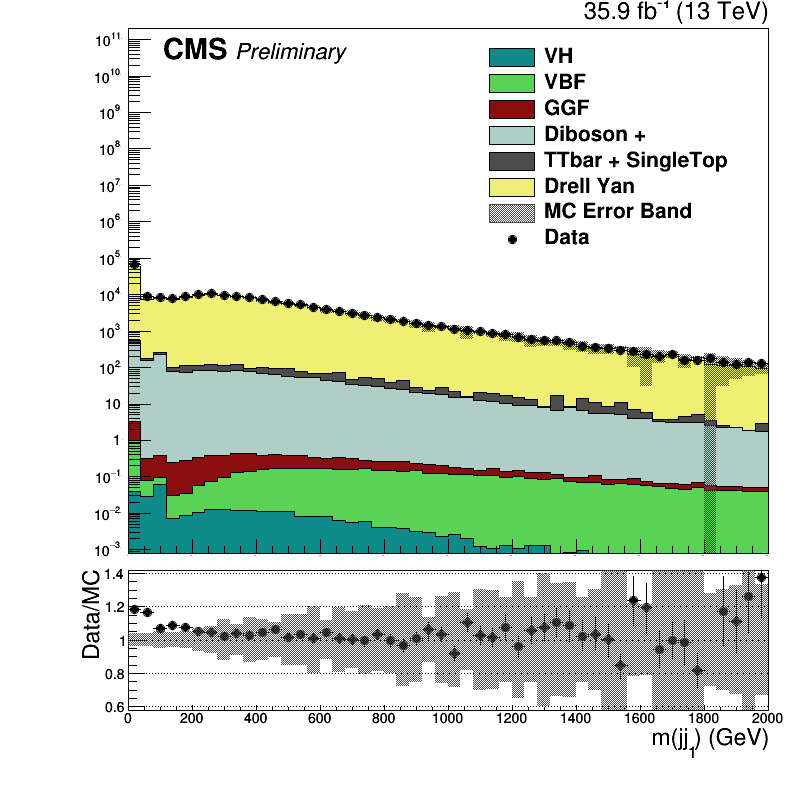
\includegraphics[width=0.32\linewidth]{images/bdt_cats/dijet1_mass_c14.png}
  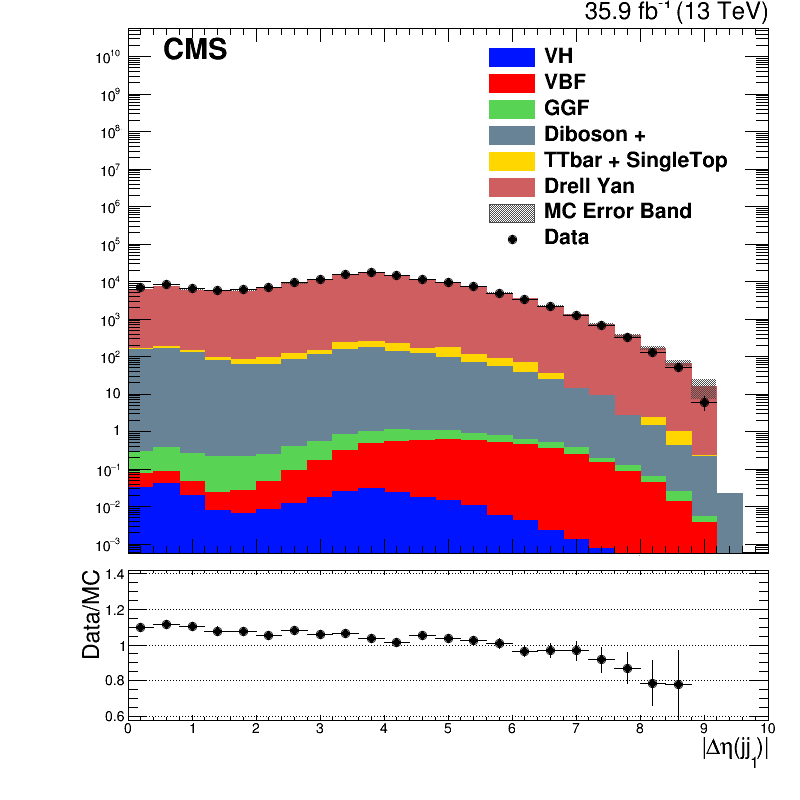
\includegraphics[width=0.32\linewidth]{images/bdt_cats/dijet1_abs_dEta_c14.png}
  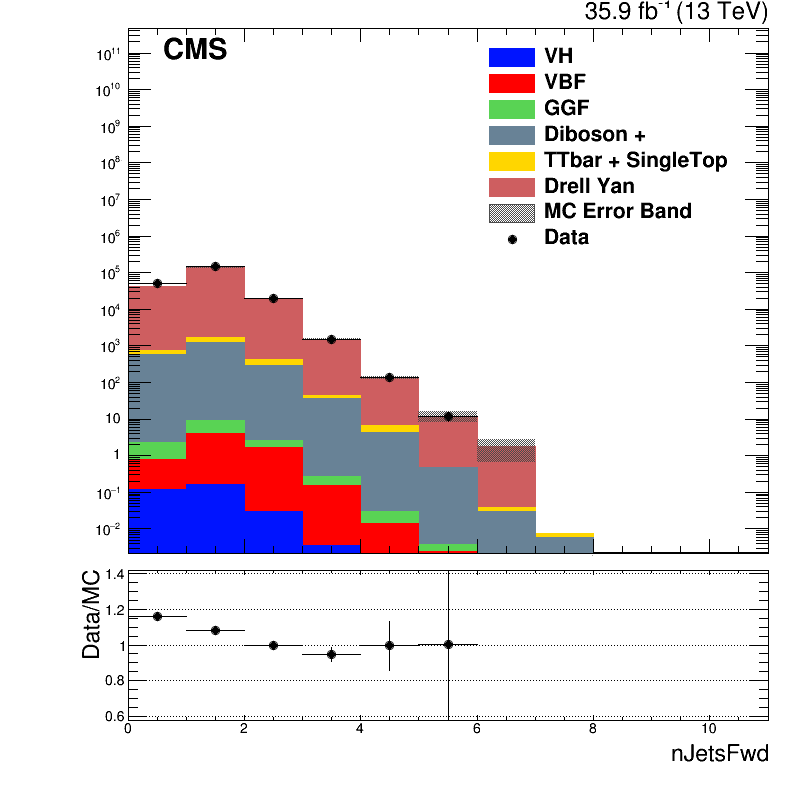
\includegraphics[width=0.32\linewidth]{images/bdt_cats/nJetsFwd_c14.png}
  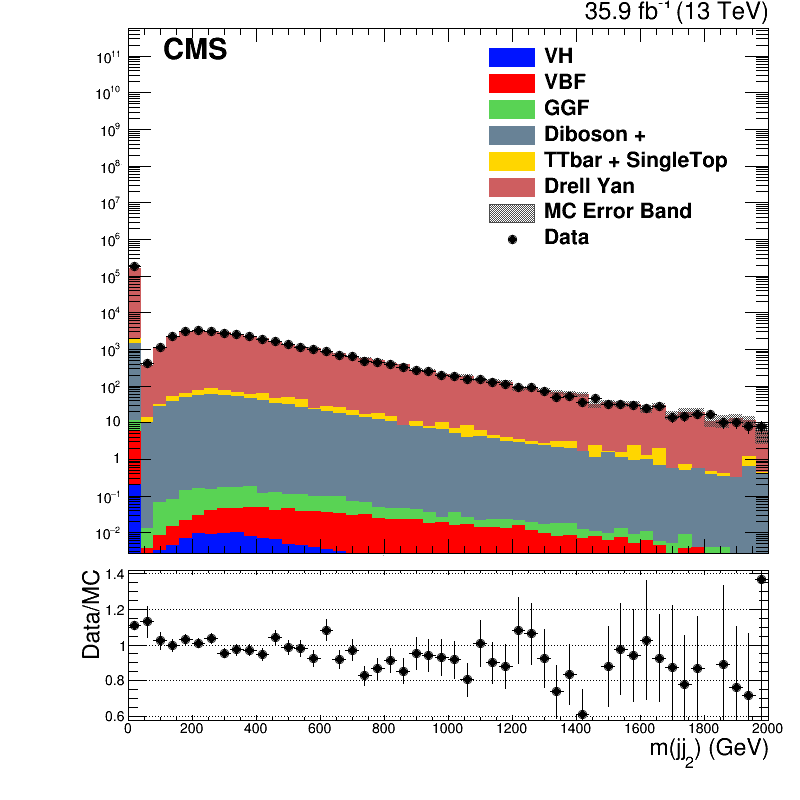
\includegraphics[width=0.32\linewidth]{images/bdt_cats/dijet2_mass_c14.png}
  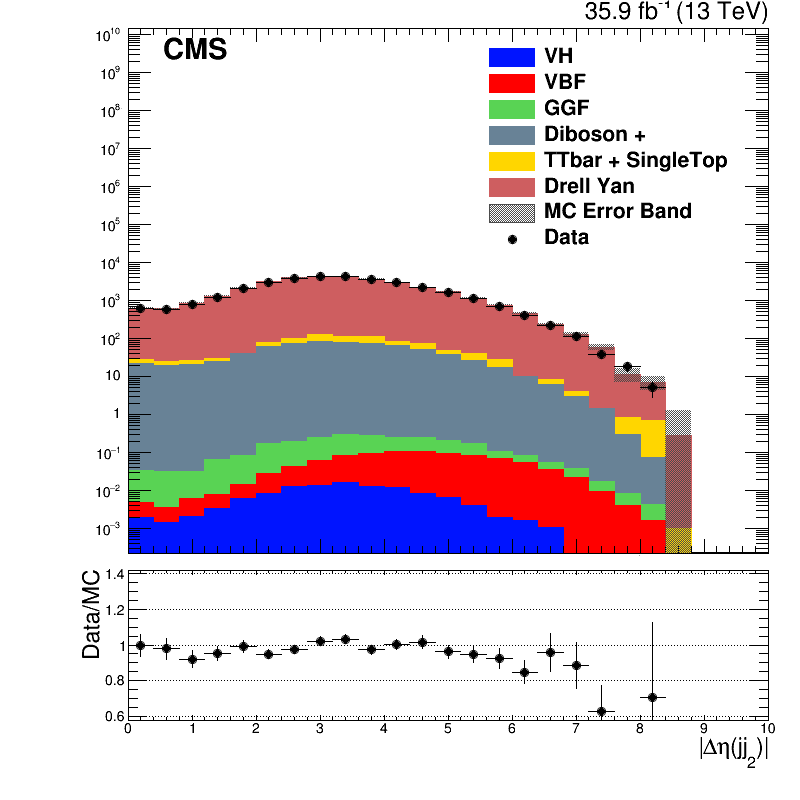
\includegraphics[width=0.32\linewidth]{images/bdt_cats/dijet2_abs_dEta_c14.png}
  \caption[Data/MC agreement for the most sensitivty category.]
   {Data/MC agreement for the most sensitive category.}
  \label{fig:valid_bdt_c14a}
\end{figure}

\begin{figure}[h!]
  \centering
  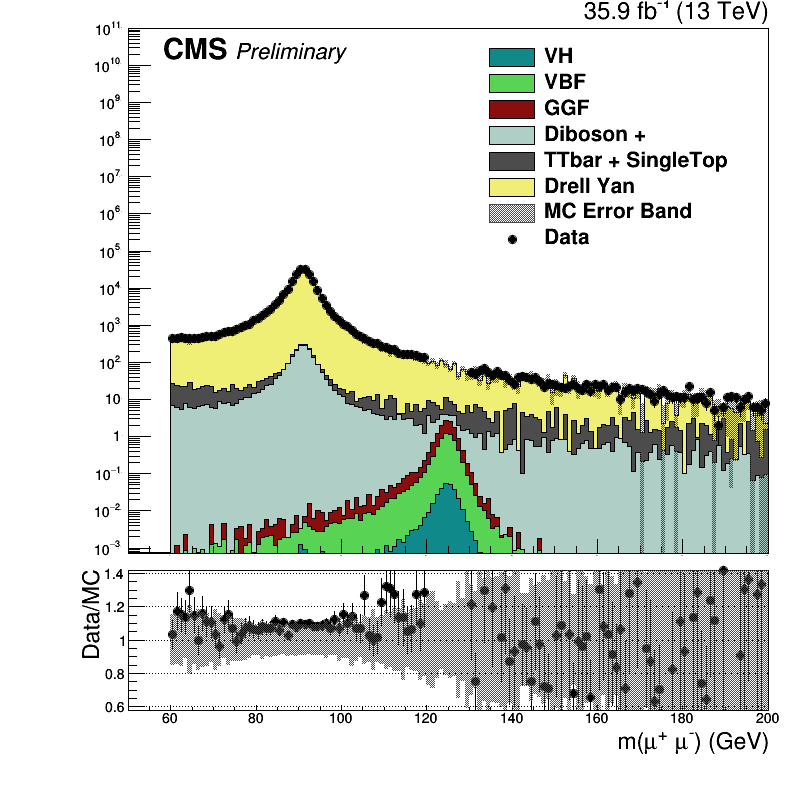
\includegraphics[width=0.32\linewidth]{images/bdt_cats/dimu_mass_Roch_c14.png}
  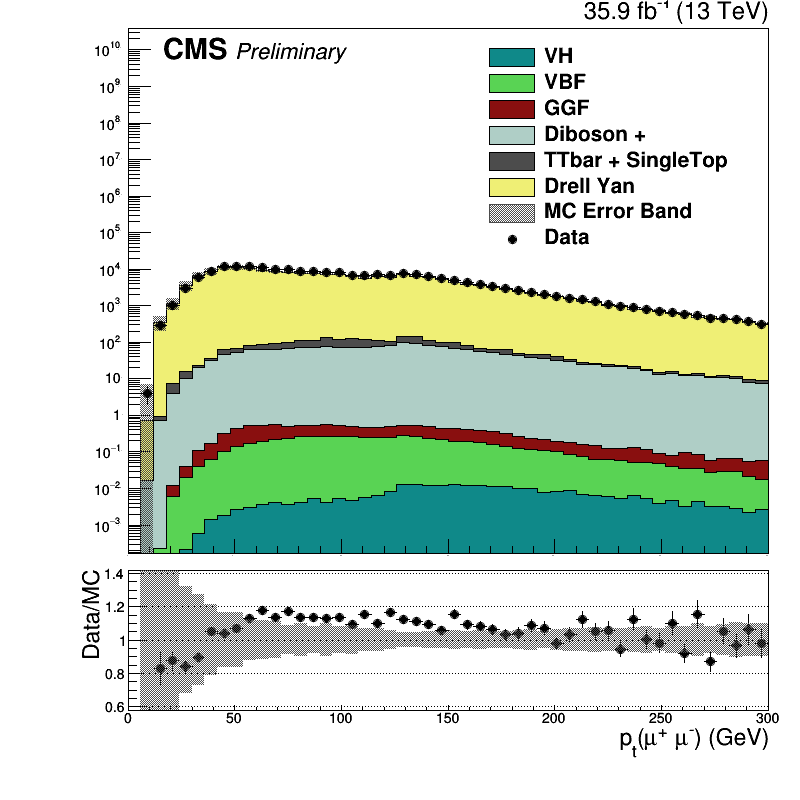
\includegraphics[width=0.32\linewidth]{images/bdt_cats/dimu_pt_c14.png}
  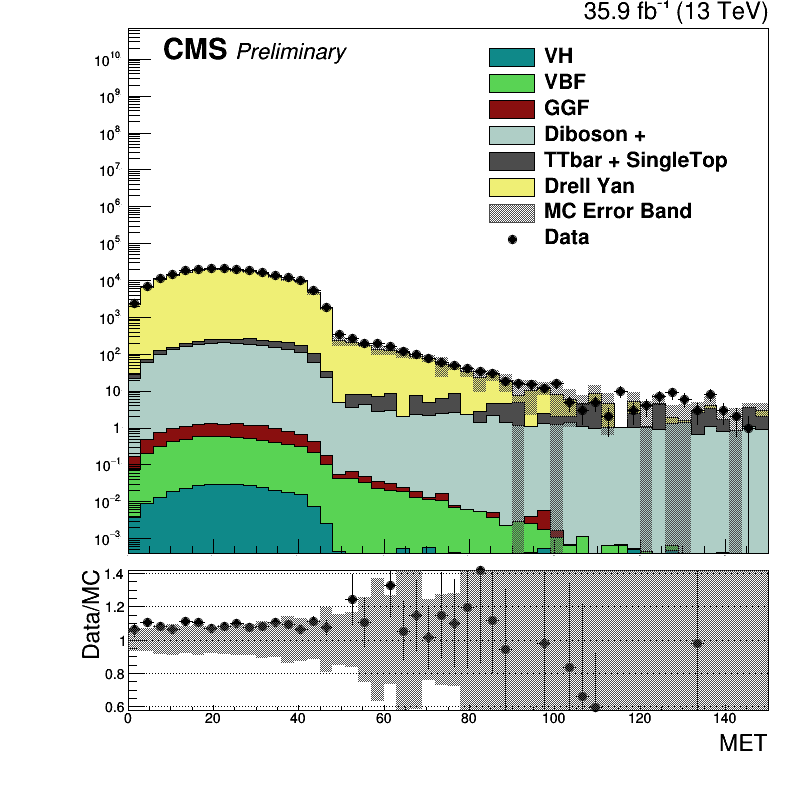
\includegraphics[width=0.32\linewidth]{images/bdt_cats/MET_c14.png}
  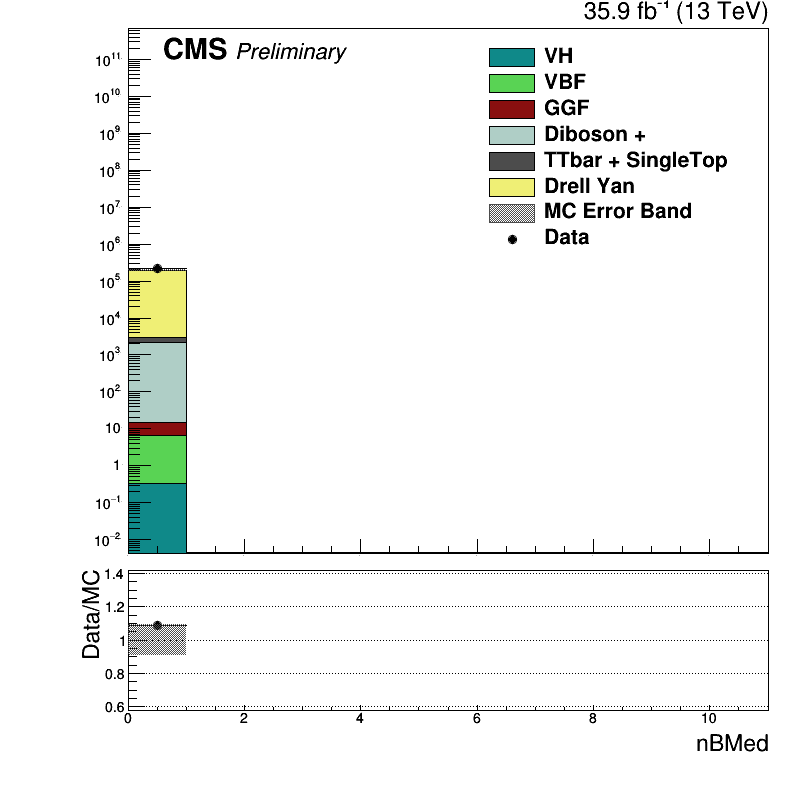
\includegraphics[width=0.32\linewidth]{images/bdt_cats/nBMed_c14.png}
  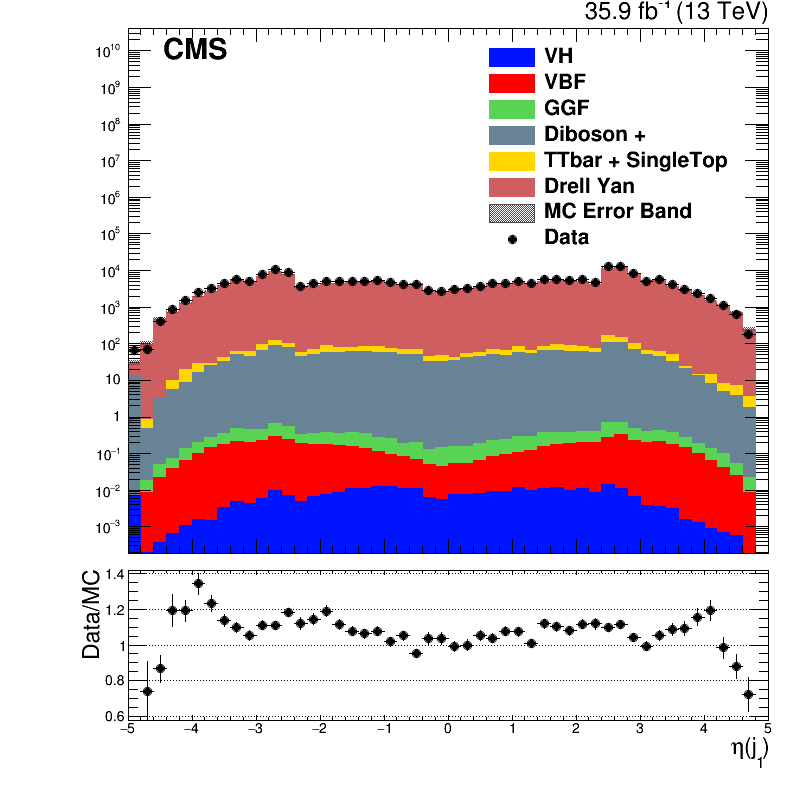
\includegraphics[width=0.32\linewidth]{images/bdt_cats/jet1_eta_c14.png}
  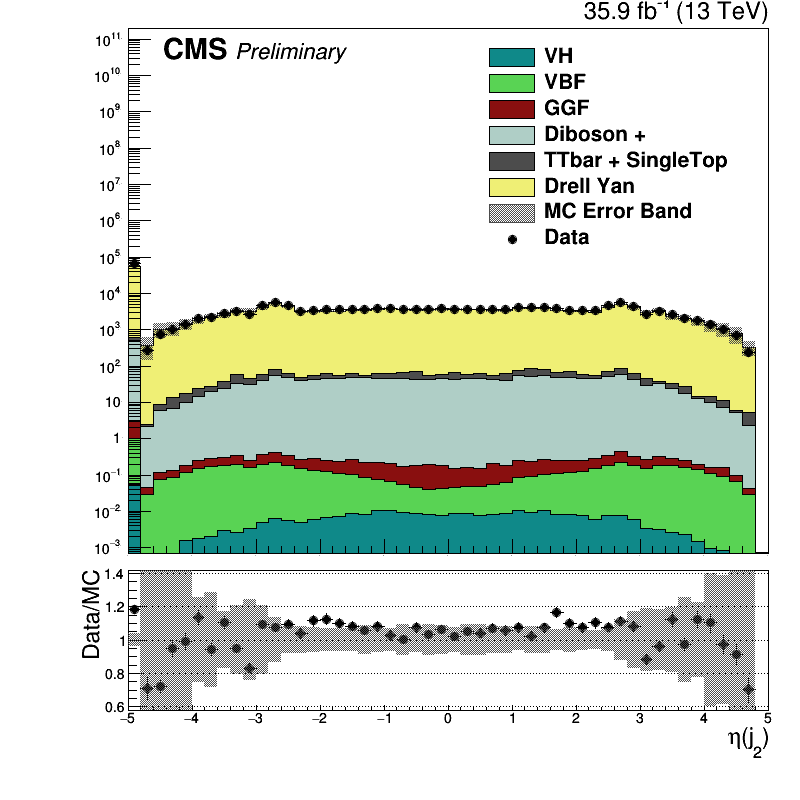
\includegraphics[width=0.32\linewidth]{images/bdt_cats/jet2_eta_c14.png}
  \caption[Additional Data/MC agreement plots for the most sensitive category.]
   {Data/MC agreement for the most sensitive category.}
  \label{fig:valid_bdt_c14b}
\end{figure}

\begin{figure}[h!]
\centering
   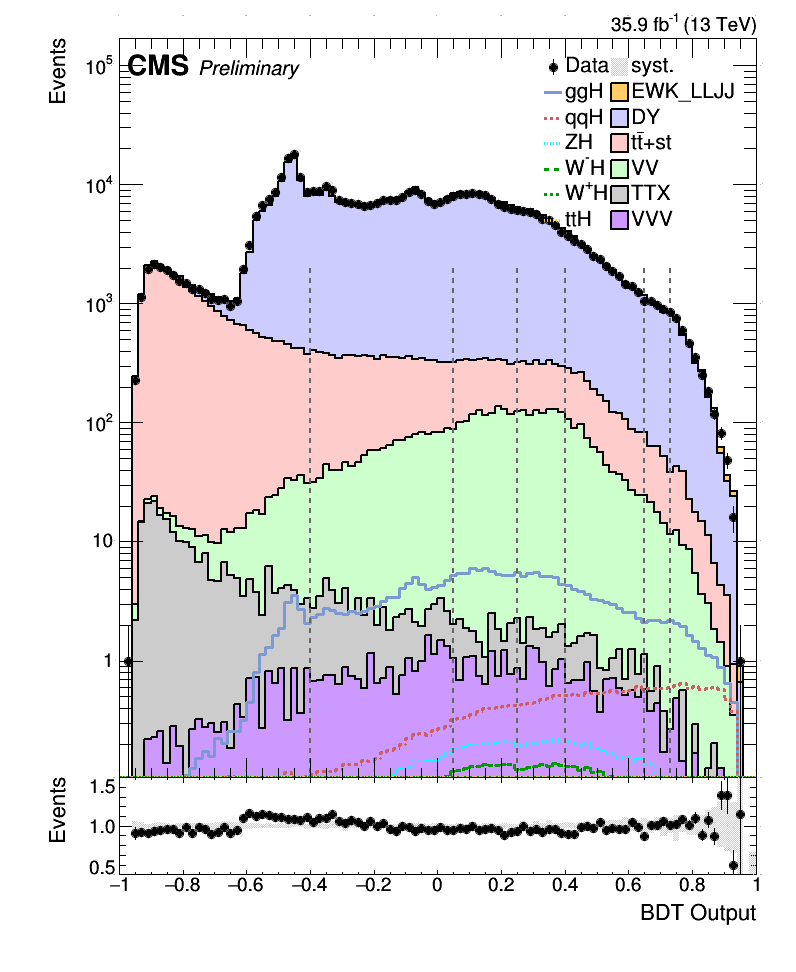
\includegraphics[width=0.49\linewidth]{images/bdt_cats/BdtOnH_bkg}
   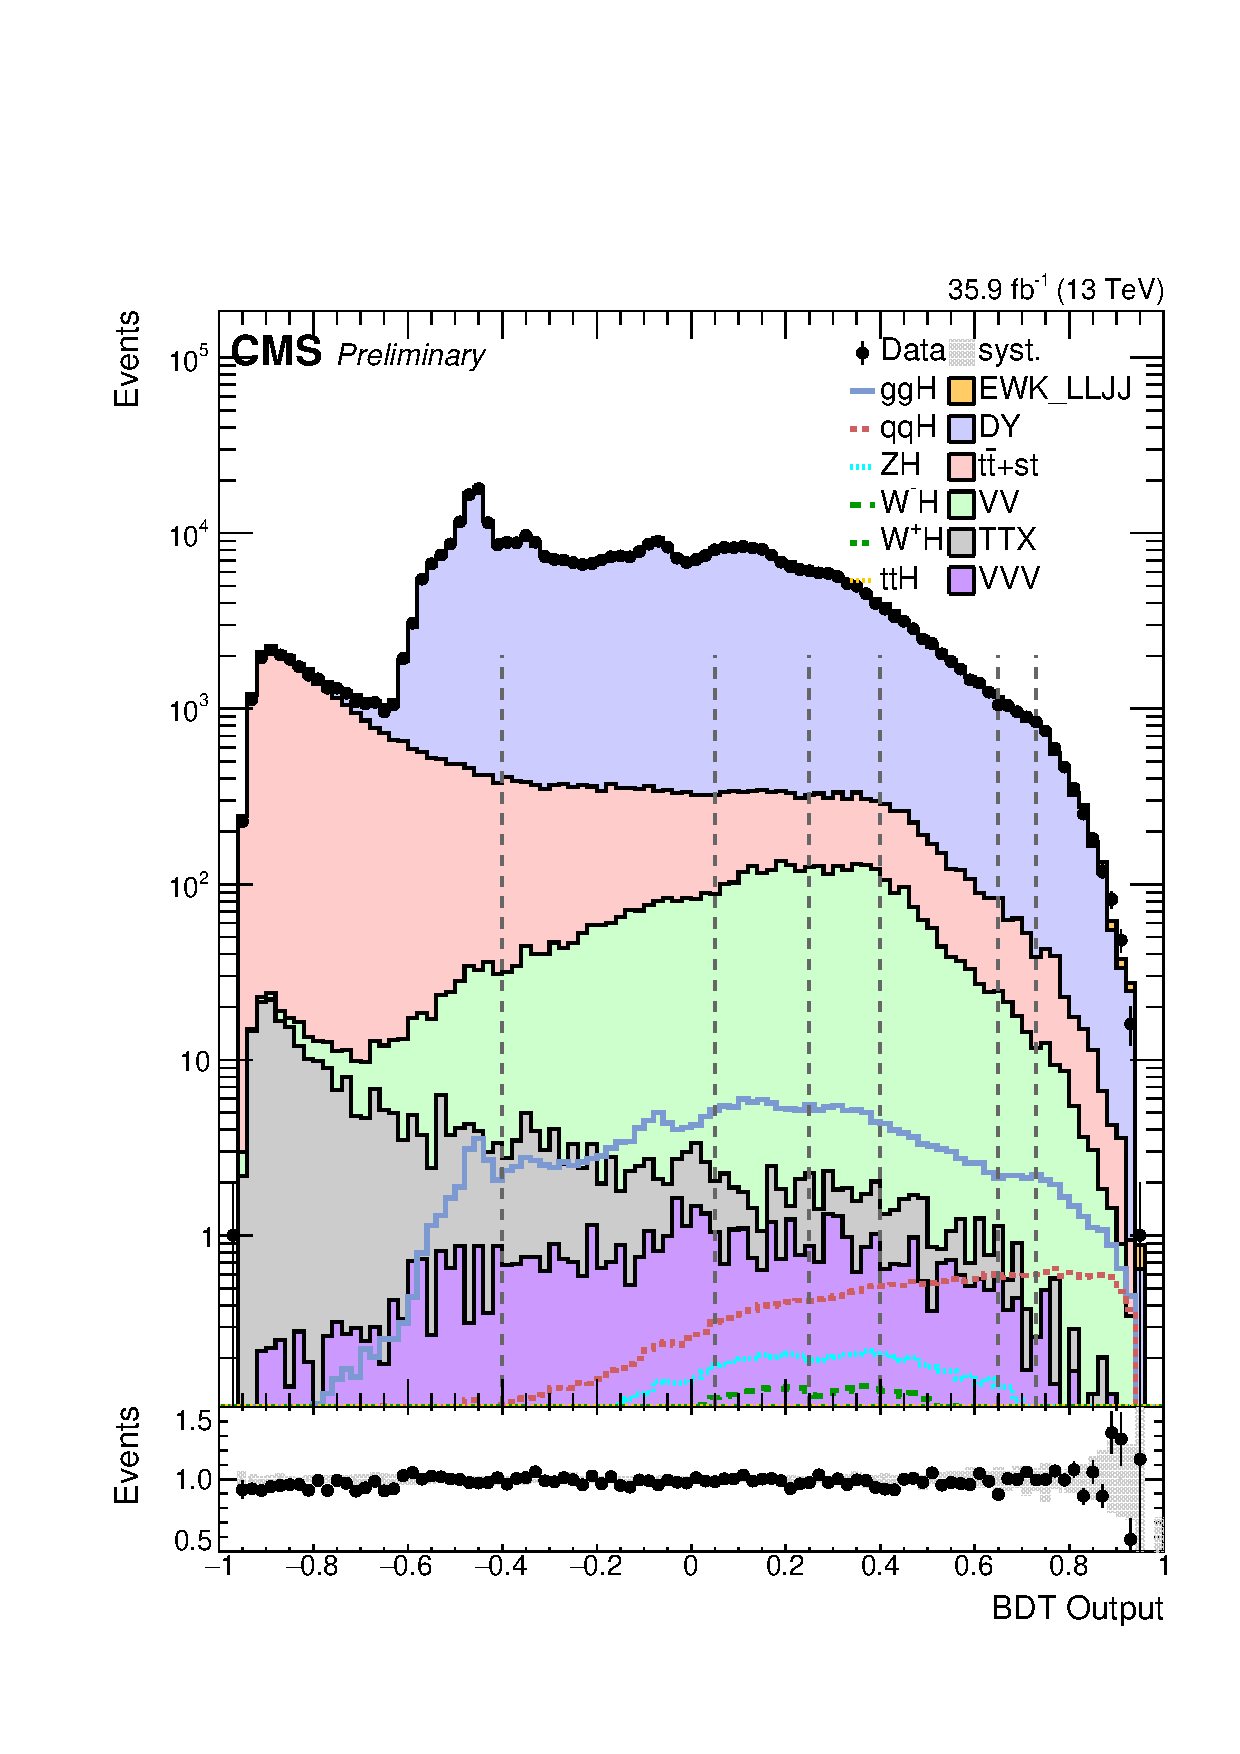
\includegraphics[width=0.49\linewidth]{images/bdt_cats/BdtOnH_zptrwg_bkg}
   \caption[The BDT score distribution in data and MC.]
   {The BDT distribution in data and MC. Right plot has DY MC with $p_t$ corrections to improve Data/MC agreement.}
  \label{fig:bdt_zpt}
\end{figure}

\begin{figure}[h!]
\centering
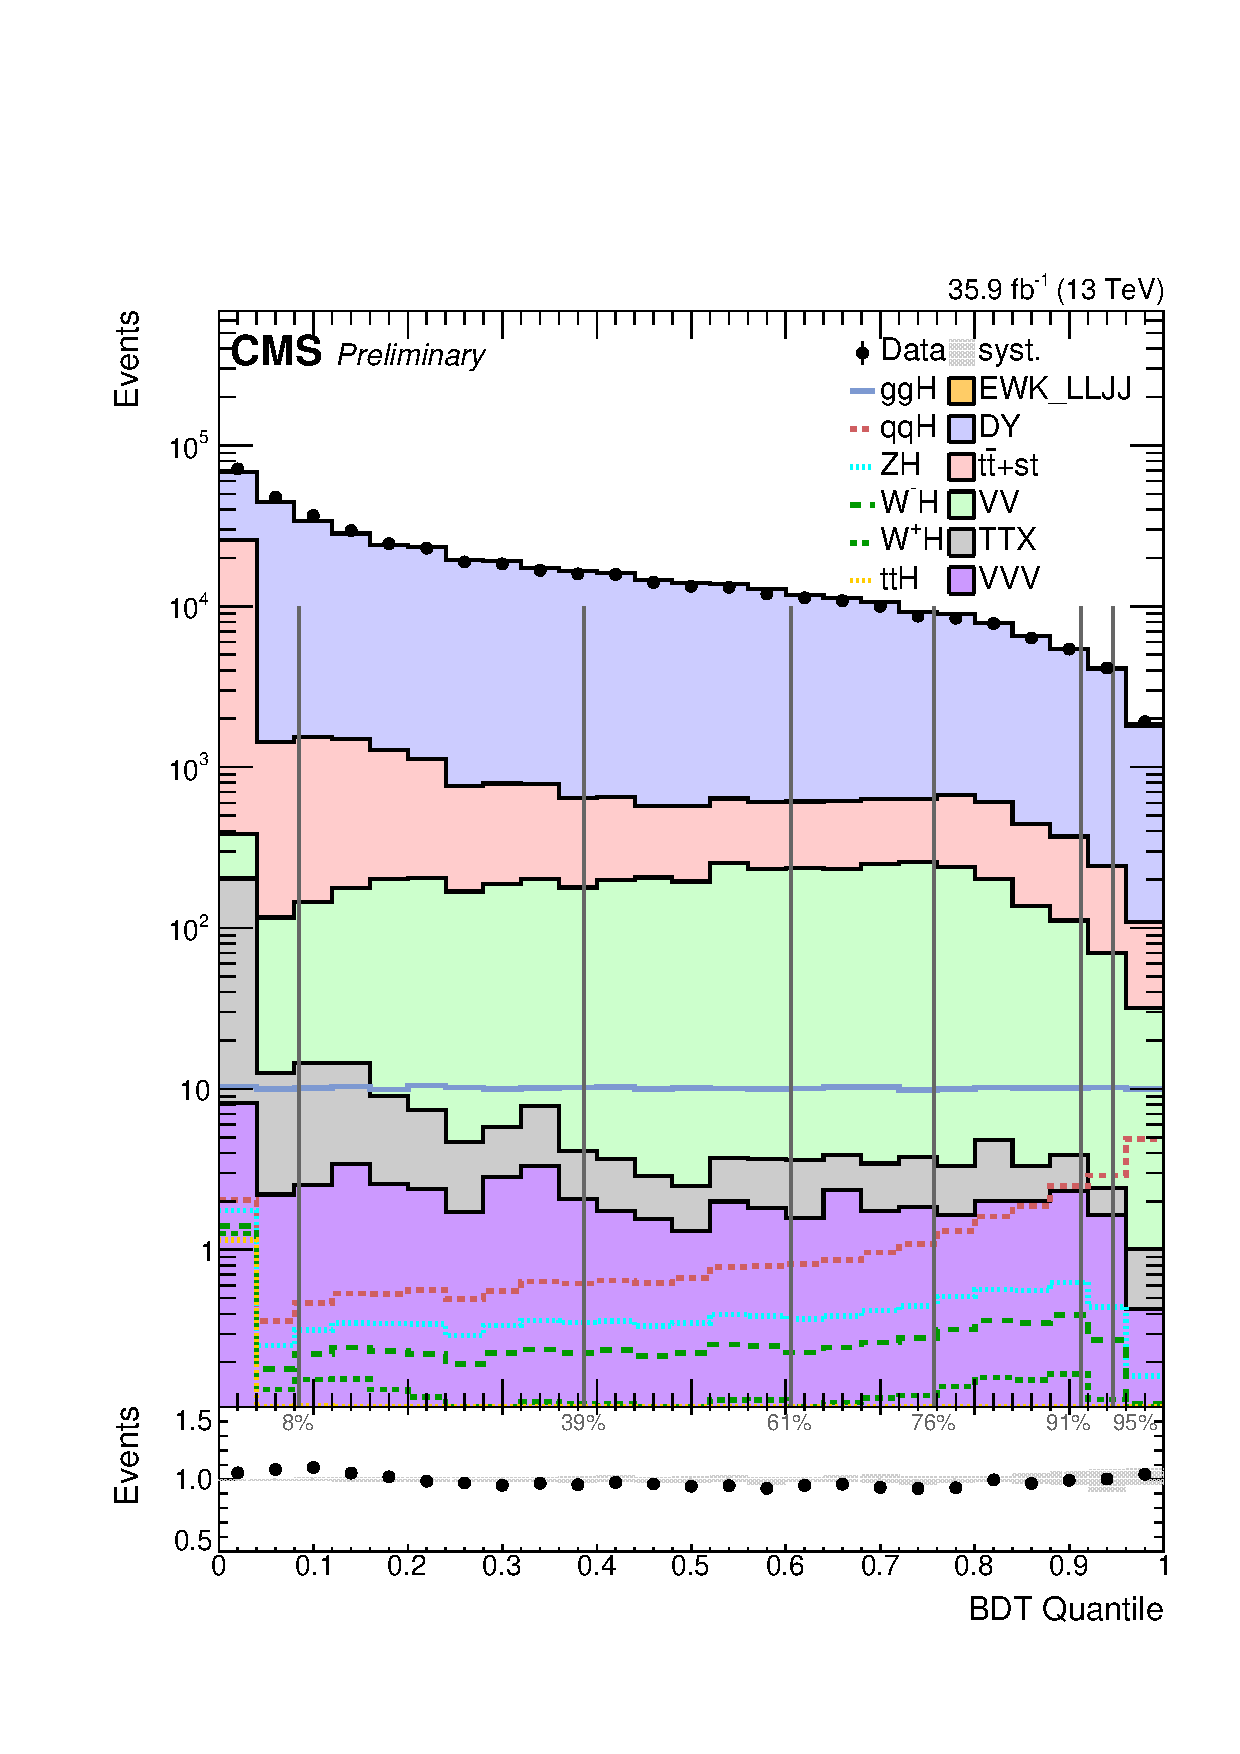
\includegraphics[width=0.5\linewidth]{images/bdt_cats/BdtOnH_QM_bkg}
  \caption[The BDT distribution in data and MC by quantile.]
  {The BDT distribution in quantile in data and MC. The systematic uncertainty is given by the JES and PU.}
  \label{fig:bdt_quantile}
\end{figure}

Lastly, it is important that the BDT score is mass independent. One way to
show this is to demonstrate that the classifier score remains the same for signal MC with different values of
$m_H$. If the BDT score does not change as the mass changes, then it is clearly mass independent. As shown in
Figure~\ref{fig:mass_independence}, the BDT score does not change significantly with the dimuon mass.

\begin{figure}[h!]
  \centering
  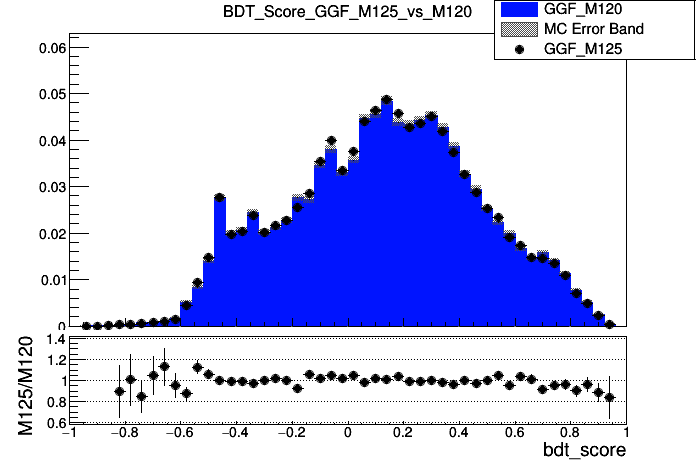
\includegraphics[width=0.49\linewidth]{images/bdt_cats/BDT_Score_GGF_M125_vs_M120.png}
  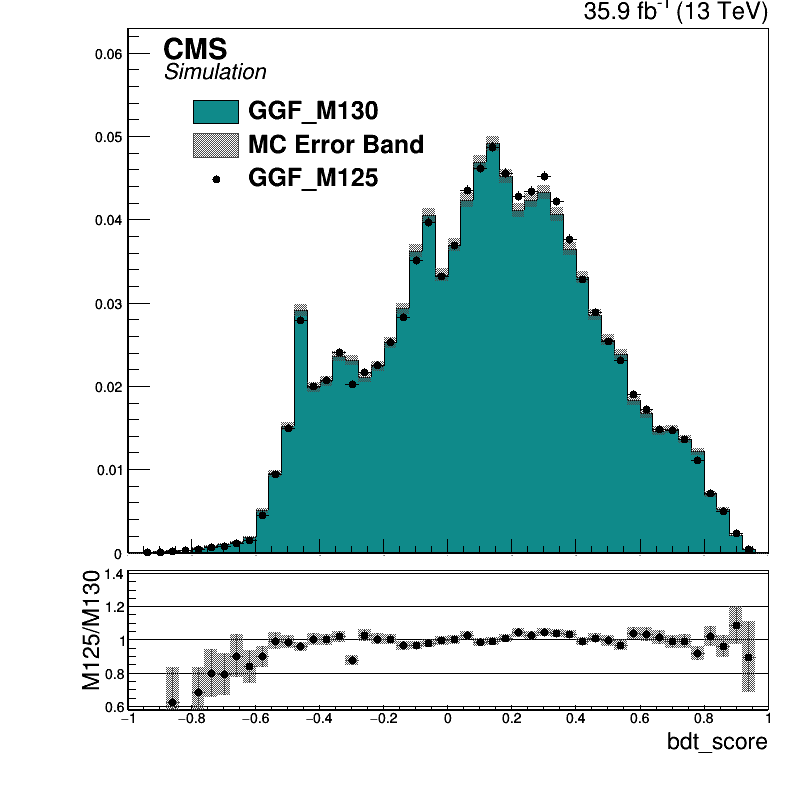
\includegraphics[width=0.49\linewidth]{images/bdt_cats/BDT_Score_GGF_M125_vs_M130.png}
  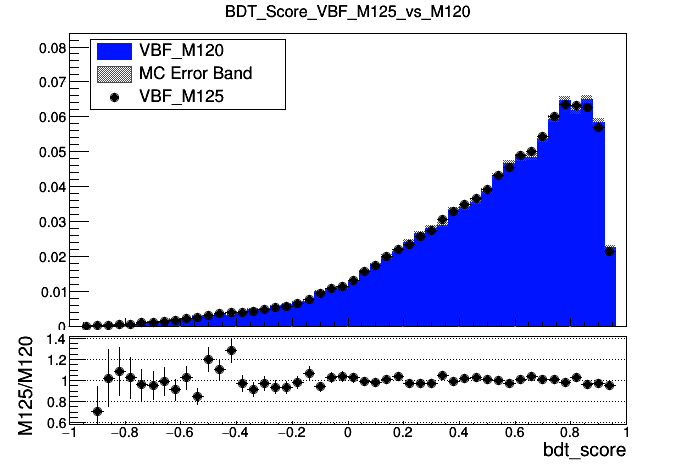
\includegraphics[width=0.49\linewidth]{images/bdt_cats/BDT_Score_VBF_M125_vs_M120.png}
  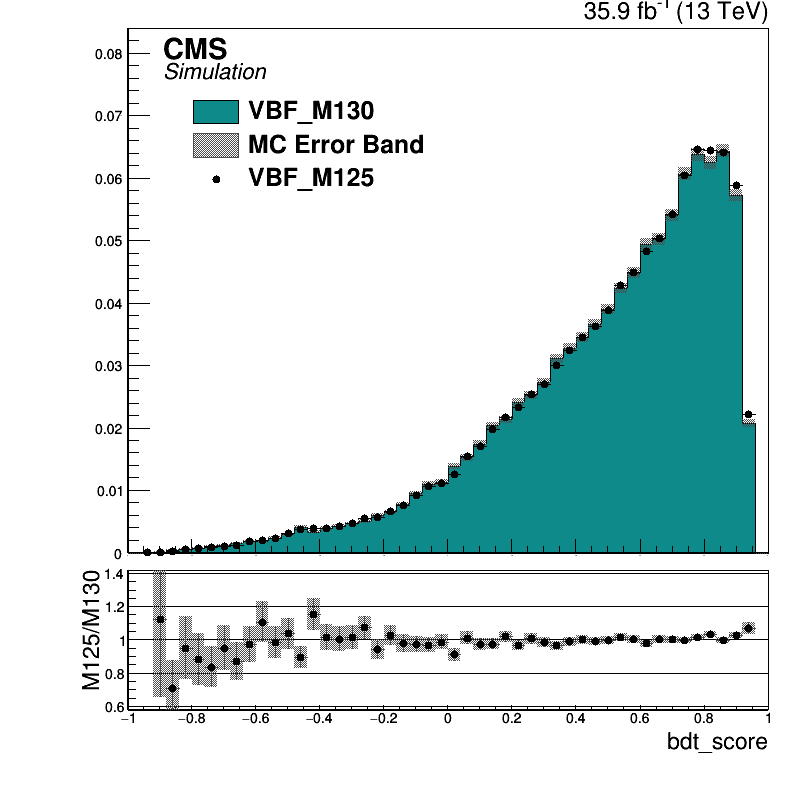
\includegraphics[width=0.49\linewidth]{images/bdt_cats/BDT_Score_VBF_M125_vs_M130.png}
  \caption[BDT mass independence plots.]
   {Plots showing the agreement between $m_H = 125\,$GeV vs. $120\,$GeV and $m_H = 125\,$GeV vs. $130\,$GeV for ggH and VBF.}
  \label{fig:mass_independence}
\end{figure}

\clearpage
\subsection{Signal And Background}

This section presents some plots and tables of interest for the signal and background. Table \ref{tab:sig_yields_table} breaks
down the signal yields by category and process. Then there are some plots showing the kinematic distributions and object counts for the signal.
The distributions are presented for the inclusive set of events starting with Figure \ref{fig:sig_kinematics_cAll1} and then for the most sensitive category (c14)
starting with Figure \ref{fig:sig_kinematics_c14-1}. After looking at the signal, Fig. \ref{fig:bkg_shapes} presents the background shapes in data
for each category and compares each to the inclusive shape.

\begin{table}[htb]
    \caption[Expected signal in each category.]{The total signal in each category predicted by the MC, broken down by process.}
%  \label{tab:cat_yields}
  \begin{center}
    \begin{tabular}{crrrrr}
     \hline
      Category     & All Signal &     GGF     &     VBF      &    VH       & $t\bar{t}H$ \\  %% & Signal events
      \hline
      Inclusive    &    253     &     224     &     18.0     &    9.213    &    1.94      \\
      c0           &    21.2    &     18.7    &     0.397    &    0.790    &    1.26      \\ 
      c1           &    22.3    &     21.1    &     0.504    &    0.652    &    0.050     \\ 
      c2           &    41.1    &     38.9    &     0.829    &    1.16     &    0.206     \\ 
      c3           &    12.7    &     12.0    &     0.226    &    0.356    &    0.138     \\ 
      c4           &    11.8    &     10.8    &     0.510    &    0.474    &    0.012     \\ 
      c5           &    29.2    &     27.1    &     0.961    &    1.03     &    0.051     \\ 
      c6           &    14.5    &     13.7    &     0.337    &    0.436    &    0.035     \\ 
      c7           &    5.2     &     4.40    &     0.443    &    0.313    &    0.006     \\ 
      c8           &    20.3    &     18.4    &     1.07     &    0.790    &    0.027     \\ 
      c9           &    13.1    &     12.2    &     0.464    &    0.405    &    0.025     \\ 
      c10          &    5.8     &     4.49    &     0.906    &    0.378    &    0.008     \\ 
      c11          &    20.3    &     16.6    &     2.56     &    1.08     &    0.043     \\ 
      c12          &    13.7    &     11.8    &     1.20     &    0.667    &    0.035     \\ 
      c13          &    8.6     &     6.27    &     1.90     &    0.435    &    0.019     \\ 
      c14          &    13.7    &     7.66    &     5.72     &    0.252    &    0.027     \\ 
      \hline
    \end{tabular}
  \end{center}
  \label{tab:sig_yields_table}
\end{table}

Comparing the signal kinematics in Figures \ref{fig:sig_kinematics_cAll1} through \ref{fig:sig_kinematics_cAll3} and \ref{fig:sig_kinematics_c14-1}
through \ref{fig:sig_kinematics_c14-3} notice that a high BDT score, exemplified by c14, removes
$t\bar{t}$-like events by requiring 0 btags and low MET. Aside from removing $t\bar{t}$, high BDT score also targets VBF-like events by requiring large dijet mass and large separation
in $\eta$ between the jets. Also note that a high BDT score picks out high dimuon $p_t$ since the signal processes generally have
higher dimuon $p_t$ than the background.

\begin{figure}[h!]
  \centering
  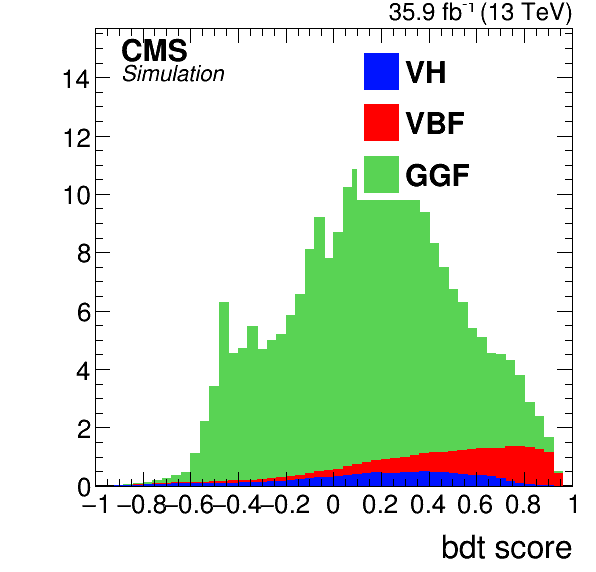
\includegraphics[width=0.32\linewidth]{images/bdt_cats/sig_kinematics_bdt_score_cAll.png}
  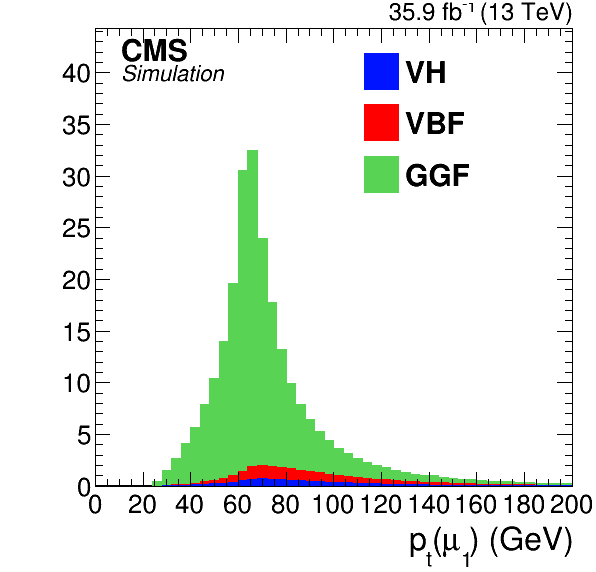
\includegraphics[width=0.32\linewidth]{images/bdt_cats/sig_kinematics_mu1_pt_cAll.png}
  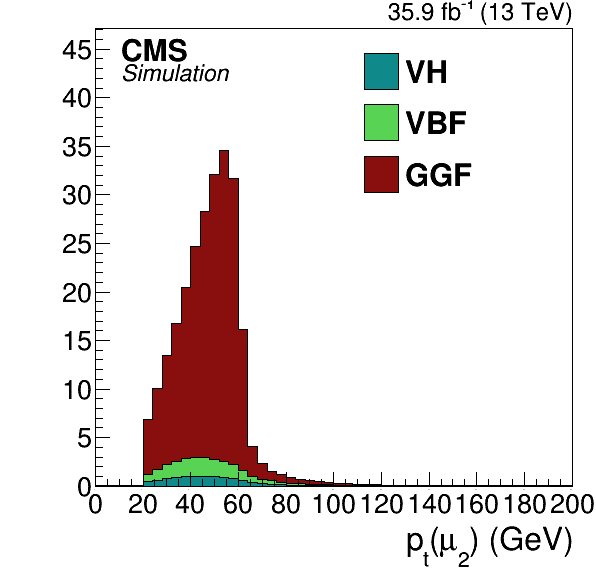
\includegraphics[width=0.32\linewidth]{images/bdt_cats/sig_kinematics_mu2_pt_cAll.png}
  \includegraphics[width=0.32\linewidth]{images/bdt_cats/sig_kinematics_mu1_eta_cAll.png}
  \includegraphics[width=0.32\linewidth]{images/bdt_cats/sig_kinematics_mu2_eta_cAll.png}
  \includegraphics[width=0.32\linewidth]{images/bdt_cats/sig_kinematics_dimu_pt_cAll.png}
  \includegraphics[width=0.32\linewidth]{images/bdt_cats/sig_kinematics_dimu_eta_cAll.png}
  \includegraphics[width=0.32\linewidth]{images/bdt_cats/sig_kinematics_dimu_abs_dPhi_cAll.png}
  \includegraphics[width=0.32\linewidth]{images/bdt_cats/sig_kinematics_dimu_abs_dEta_cAll.png}
  \caption[Kinematic and object count distributions for the inclusive signal MC.]
   {Kinematics and object counts for the signal in the inclusive set of events.}
  \label{fig:sig_kinematics_cAll1}
\end{figure}
\begin{figure}[h!]
  \includegraphics[width=0.32\linewidth]{images/bdt_cats/sig_kinematics_dimu_mass_KaMu_cAll.png}
  \includegraphics[width=0.32\linewidth]{images/bdt_cats/sig_kinematics_dijet1_mass_cAll.png}
  \includegraphics[width=0.32\linewidth]{images/bdt_cats/sig_kinematics_dijet1_abs_dEta_cAll.png}
  \includegraphics[width=0.32\linewidth]{images/bdt_cats/sig_kinematics_dijet2_mass_cAll.png}
  \includegraphics[width=0.32\linewidth]{images/bdt_cats/sig_kinematics_dijet2_abs_dEta_cAll.png}
  \includegraphics[width=0.32\linewidth]{images/bdt_cats/sig_kinematics_jet1_pt_cAll.png}
  \includegraphics[width=0.32\linewidth]{images/bdt_cats/sig_kinematics_jet2_pt_cAll.png}
  \includegraphics[width=0.32\linewidth]{images/bdt_cats/sig_kinematics_jet1_eta_cAll.png}
  \includegraphics[width=0.32\linewidth]{images/bdt_cats/sig_kinematics_jet2_eta_cAll.png}
  \caption[More kinematic and object count distributions for the inclusive signal MC.]
   {More kinematic and object count histograms for the signal in the inclusive set of events.}
  \label{fig:sig_kinematics_cAll2}
\end{figure}

\begin{figure}[h!]
  \includegraphics[width=0.32\linewidth]{images/bdt_cats/sig_kinematics_MET_cAll.png}
  \includegraphics[width=0.32\linewidth]{images/bdt_cats/sig_kinematics_nJets_cAll.png}
  \includegraphics[width=0.32\linewidth]{images/bdt_cats/sig_kinematics_nJetsCent_cAll.png}
  \includegraphics[width=0.32\linewidth]{images/bdt_cats/sig_kinematics_nBMed_cAll.png}
  \includegraphics[width=0.32\linewidth]{images/bdt_cats/sig_kinematics_nExtraMu_cAll.png}
  \includegraphics[width=0.32\linewidth]{images/bdt_cats/sig_kinematics_nEle_cAll.png}
  \caption[Even more kinematic and object count distributions for the inclusive signal MC.]
   {More kinematic and object count histograms for the signal in the inclusive set of events.}
  \label{fig:sig_kinematics_cAll3}
\end{figure}

\begin{figure}[h!]
  \centering
  \includegraphics[width=0.32\linewidth]{images/bdt_cats/sig_kinematics_bdt_score_c14.png}
  \includegraphics[width=0.32\linewidth]{images/bdt_cats/sig_kinematics_mu1_pt_c14.png}
  \includegraphics[width=0.32\linewidth]{images/bdt_cats/sig_kinematics_mu2_pt_c14.png}
  \includegraphics[width=0.32\linewidth]{images/bdt_cats/sig_kinematics_mu1_eta_c14.png}
  \includegraphics[width=0.32\linewidth]{images/bdt_cats/sig_kinematics_mu2_eta_c14.png}
  \includegraphics[width=0.32\linewidth]{images/bdt_cats/sig_kinematics_dimu_pt_c14.png}
  \includegraphics[width=0.32\linewidth]{images/bdt_cats/sig_kinematics_dimu_eta_c14.png}
  \includegraphics[width=0.32\linewidth]{images/bdt_cats/sig_kinematics_dimu_abs_dPhi_c14.png}
  \includegraphics[width=0.32\linewidth]{images/bdt_cats/sig_kinematics_dimu_abs_dEta_c14.png}
  \caption[Kinematic and object count distributions for the signal MC in the most sensitive category.]
   {Kinematic and object count histograms for the signal in category c14. Note the high dimuon $p_t$ targeting the signal in general.}
  \label{fig:sig_kinematics_c14-1}
\end{figure}

\begin{figure}[h!]
  \includegraphics[width=0.32\linewidth]{images/bdt_cats/sig_kinematics_dimu_mass_KaMu_c14.png}
  \includegraphics[width=0.32\linewidth]{images/bdt_cats/sig_kinematics_dijet1_mass_c14.png}
  \includegraphics[width=0.32\linewidth]{images/bdt_cats/sig_kinematics_dijet1_abs_dEta_c14.png}
  \includegraphics[width=0.32\linewidth]{images/bdt_cats/sig_kinematics_dijet2_mass_c14.png}
  \includegraphics[width=0.32\linewidth]{images/bdt_cats/sig_kinematics_dijet2_abs_dEta_c14.png}
  \includegraphics[width=0.32\linewidth]{images/bdt_cats/sig_kinematics_jet1_pt_c14.png}
  \includegraphics[width=0.32\linewidth]{images/bdt_cats/sig_kinematics_jet2_pt_c14.png}
  \includegraphics[width=0.32\linewidth]{images/bdt_cats/sig_kinematics_jet1_eta_c14.png}
  \includegraphics[width=0.32\linewidth]{images/bdt_cats/sig_kinematics_jet2_eta_c14.png}
  \caption[More kinematic and object count distributions for the signal MC in the most sensitive category.]
   {More kinematic and object count histograms for the signal in category c14. Note large dijet mass and the large separation in eta for the jets
    targeting VBF.}
  \label{fig:sig_kinematics_c14-2}
\end{figure}
\begin{figure}[h!]
  \includegraphics[width=0.32\linewidth]{images/bdt_cats/sig_kinematics_MET_c14.png}
  \includegraphics[width=0.32\linewidth]{images/bdt_cats/sig_kinematics_nJets_c14.png}
  \includegraphics[width=0.32\linewidth]{images/bdt_cats/sig_kinematics_nJetsCent_c14.png}
  \includegraphics[width=0.32\linewidth]{images/bdt_cats/sig_kinematics_nJetsFwd_c14.png}
  \includegraphics[width=0.32\linewidth]{images/bdt_cats/sig_kinematics_nBMed_c14.png}
  \includegraphics[width=0.32\linewidth]{images/bdt_cats/sig_kinematics_nExtraMu_c14.png}
  \includegraphics[width=0.32\linewidth]{images/bdt_cats/sig_kinematics_nEle_c14.png}
  \caption[Even more kinematic and object count distributions for the signal MC in the most sensitive category.]
   {More kinematic and object count histograms for the signal in category c14. Note the low MET and 0 btags which exclude $t\bar{t}$.}
  \label{fig:sig_kinematics_c14-3}
\end{figure}

The factors influencing the shape of the background are the mass resolution (determined by muon $\eta$) and the BDT score. High resolution (low muon $\eta$)
categories will have a narrower Z peak with more events proportionally
on the high side of the Z peak---lower mass on the plots shown in Fig. \ref{fig:bkg_shapes}.
See c9 as an example. A high BDT score has a similar effect: since there are fewer $t\bar{t}$ like events, there are proportionally
more events at lower mass than in the tail. See c14 for this effect. In Figure \ref{fig:bkg_shapes}, the background shape for each category
is normalized and compared to the inclusive set of events so that it's easy to compare the variation in shape between categories.

\begin{figure}[h!]
  \centering
  \includegraphics[width=0.25\linewidth]{images/bdt_cats/bkg_shapes_stack_c0.png}
  \includegraphics[width=0.25\linewidth]{images/bdt_cats/bkg_shapes_stack_c1.png}
  \includegraphics[width=0.25\linewidth]{images/bdt_cats/bkg_shapes_stack_c2.png}
  \includegraphics[width=0.25\linewidth]{images/bdt_cats/bkg_shapes_stack_c3.png}
  \includegraphics[width=0.25\linewidth]{images/bdt_cats/bkg_shapes_stack_c4.png}
  \includegraphics[width=0.25\linewidth]{images/bdt_cats/bkg_shapes_stack_c5.png}
  \includegraphics[width=0.25\linewidth]{images/bdt_cats/bkg_shapes_stack_c6.png}
  \includegraphics[width=0.25\linewidth]{images/bdt_cats/bkg_shapes_stack_c7.png}
  \includegraphics[width=0.25\linewidth]{images/bdt_cats/bkg_shapes_stack_c8.png}
  \includegraphics[width=0.25\linewidth]{images/bdt_cats/bkg_shapes_stack_c9.png}
  \includegraphics[width=0.25\linewidth]{images/bdt_cats/bkg_shapes_stack_c10.png}
  \includegraphics[width=0.25\linewidth]{images/bdt_cats/bkg_shapes_stack_c11.png}
  \includegraphics[width=0.25\linewidth]{images/bdt_cats/bkg_shapes_stack_c13.png}
  \includegraphics[width=0.25\linewidth]{images/bdt_cats/bkg_shapes_stack_c14.png}
  \caption[Background shapes in data in the different categories.]
   {The difference in background shapes between the categories in data. The plots show the data with the signal region blinded.
    Each category's background shape is compared to the inclusive shape.}
  \label{fig:bkg_shapes}
\end{figure}
